\documentclass[]{article}
\usepackage{amsfonts}
\usepackage{amsmath}
\usepackage{amssymb}
\usepackage{graphicx}
\usepackage{amsthm}
\usepackage{svg}
\usepackage{enumitem}
\usepackage{color}
\usepackage{float}
\usepackage[utf8]{inputenc}
\usepackage{wrapfig}
\usepackage[arrow]{xy}
\usepackage{tikz-cd}



%%%%% Alphabets %%%%% 
\def\cA{\mathcal{A}}\def\cB{\mathcal{B}}\def\cC{\mathcal{C}}\def\cD{\mathcal{D}}\def\cE{\mathcal{E}}\def\cF{\mathcal{F}}\def\cG{\mathcal{G}}\def\cH{\mathcal{H}}\def\cI{\mathcal{I}}\def\cJ{\mathcal{J}}\def\cK{\mathcal{K}}\def\cL{\mathcal{L}}\def\cM{\mathcal{M}}\def\cN{\mathcal{N}}\def\cO{\mathcal{O}}\def\cP{\mathcal{P}}\def\cQ{\mathcal{Q}}\def\cR{\mathcal{R}}\def\cS{\mathcal{S}}\def\cT{\mathcal{T}}\def\cU{\mathcal{U}}\def\cV{\mathcal{V}}\def\cW{\mathcal{W}}\def\cX{\mathcal{X}}\def\cY{\mathcal{Y}}\def\cZ{\mathcal{Z}}

\def\AA{\mathbb{A}} \def\BB{\mathbb{B}} \def\CC{\mathbb{C}} \def\DD{\mathbb{D}} \def\EE{\mathbb{E}} \def\FF{\mathbb{F}} \def\GG{\mathbb{G}} \def\HH{\mathbb{H}} \def\II{\mathbb{I}} \def\JJ{\mathbb{J}} \def\KK{\mathbb{K}} \def\LL{\mathbb{L}} \def\MM{\mathbb{M}} \def\NN{\mathbb{N}} \def\OO{\mathbb{O}} \def\PP{\mathbb{P}} \def\QQ{\mathbb{Q}} \def\RR{\mathbb{R}} \def\SS{\mathbb{S}} \def\TT{\mathbb{T}} \def\UU{\mathbb{U}} \def\VV{\mathbb{V}} \def\WW{\mathbb{W}} \def\XX{\mathbb{X}} \def\YY{\mathbb{Y}} \def\ZZ{\mathbb{Z}}  

\def\bU{\mathbf{U}} \def\btU{\tilde{\bU}} \def\bUs{\bU^\circ}
\def\btUos{\btU_0^\circ}
\def\bG{\mathbf{G}} \def\bGs{\mathbf{G}^\circ}
\def\hol{\mathbf{hol}}
\def\bM{\mathbf{M}}
\def\bMs{\mathbf{M}^\circ}
\def\btUs{\btU^\circ} 
\def\xtild{\tilde{x}_0}
\def\utild{\tilde{u}_0}
\def\mtild{\tilde{m}_0}
\def\gamtild{\tilde{\gamma}}
\def\phitild{\tilde{\Phi}}
\def\tildphi{\tilde{\phi}}

\def\fa{\mathfrak{a}} \def\fb{\mathfrak{b}} \def\fc{\mathfrak{c}} \def\fd{\mathfrak{d}} \def\fe{\mathfrak{e}} \def\ff{\mathfrak{f}} \def\fg{\mathfrak{g}} \def\fh{\mathfrak{h}} \def\fj{\mathfrak{j}} \def\fk{\mathfrak{k}} \def\fl{\mathfrak{l}} \def\fm{\mathfrak{m}} \def\fn{\mathfrak{n}} \def\fo{\mathfrak{o}} \def\fp{\mathfrak{p}} \def\fq{\mathfrak{q}} \def\fr{\mathfrak{r}} \def\fs{\mathfrak{s}} \def\ft{\mathfrak{t}} \def\fu{\mathfrak{u}} \def\fv{\mathfrak{v}} \def\fw{\mathfrak{w}} \def\fx{\mathfrak{x}} \def\fy{\mathfrak{y}} \def\fz{\mathfrak{z}}
\def\fgl{\mathfrak{gl}}  \def\fsl{\mathfrak{sl}}  \def\fso{\mathfrak{so}}  \def\fsp{\mathfrak{sp}}  
\def\GL{\mathrm{GL}} \def\SL{\mathrm{SL}}  \def\SP{\mathrm{SL}}
\def\SO{\mathrm{SO}}

\def\<{\langle} \def\>{\rangle}
\def\ad{\mathrm{ad}} 
\def\Aut{\mathrm{Aut}}
\def\dim{\mathrm{dim}} 
\def\End{\mathrm{End}} 
\def\ev{\mathrm{ev}} 
\def\half{\hbox{$\frac12$}}
\def\Hom{\mathrm{Hom}} 
\def\qtr{\mathrm{qtr}} 
\def\tr{\mathrm{tr}} 
\def\Tr{\mathrm{Tr}} 
\def\vep{\varepsilon}

\def\ZZn{\ZZ/n\ZZ}
\def\acts{\rotatebox[origin=c]{-90}{$\circlearrowright$}}
%%%%%%%%%%%%%%%%%%%%%%%%%%%%%% 
%%%%%%%%%%%%%%%%%%%%%%%%%%%%%%


\begin{document}
\newtheorem{thm}{Theorem}[]
\newtheorem{Def}{Definition}[]
\newtheorem*{thm*}{Theorem}
\newtheorem*{def*}{Definition}
\newtheorem{lem}{Lemma}
\newtheorem*{rem}{Remark}
\newcommand{\shiftleft}[2]{\makebox[0pt][r]{\makebox[#1][l]{#2}}}
\newtheorem*{conj}{Conjecture}
\newtheorem{cor}{Corollary}[]

\newcommand{\compav}[1]{\textbf{\textcolor{blue}{#1}}}
\newcommand{\compat}[1]{\textbf{\textcolor{red}{#1}}}
\graphicspath{{images/}}
\setsvg{svgpath={./images/}}

% Title Page


\title{Periodicity of Geodesics on the Necker Cube Surface}
\author{Pavel Javornik}

\maketitle

%\begin{center}
%
%\includesvg[width=4.8in]{cubecoverphoto}\\
%\end{center}

\begin{abstract}
\noindent Although it is most recognizable as M.C. Escher's adaptation of an optical illusion popularized by Louis Albert Necker, the Necker cube surface has a complex structure and is, in analaytic language, described as an infinite, flat (locally isometric to $\RR^2$ on smooth sections), $\RR^3$-embeddable Euclidean cone surface with countably many singularities of cone angles $3\pi$ and $\frac{3\pi}{2}$. Its geometric construction is described as the gluing of infinitely many unit cubes along their edges so that every face shares an edge with exactly four others. A unit-speed geodesic on this surface has an initial trajectory angle $\theta\in\RR/2\pi\ZZ$ given up by the surface's local plane isometry. Given a rational vector direction in $\RR^2$ (components are relatively prime integers) obtained from $\theta$, one can classify every periodic/drift-periodic rational geodesic on the surface. In addition its total period/length and, in the case where it is drift-periodic, translational drift as Euclidean distance in its ambient space is given by solving a system of Diophantine equations seemingly related to Farey sequences.
\end{abstract}
\begin{figure}[H]
\centering
\includesvg[width=4in]{cubesxyzpaths2bwv2b}
\label{fig:front}
\caption{Periodic and drift-periodic geodesics on the Necker cube surface}
\end{figure}
\section{Introduction}
The Necker cube has made numerous appearances in the work of mathematicians, crystallographers, and scientists interested in human visual systems even before appearing in the works of M.C. Escher [cite]. Louis Albert Necker was credited for having discovered this optical illusion and studying its various properties [cite]. The solid presentation of the cube, when rendered as a flat surface with three rear faces removed, achieves a similar effect when its three visible faces are shaded in a particular way not unlike the illusion given off by the ``wire-frame" cube.[cite] The Necker cube surface is then obtained by gluing infinitely many copies of the semi-cube surface along its outer edges (Fig 1).


Dynamical classification of geodesics on flat, infinite surfaces admitting cone singularities such as the Necker cube surface ultimately boils down to studying the surface's and, if it exists, base surface's various symmetries. The rotational holonomy group acts on the unit tangent bundle of the surface as a unit vector (derivative of the geodesic at any given time) undergoes parallel transport along the geodesic path. If a surface is periodically constructed and obtained as a normal cover of some elementary base surface (like a polygon with edge identifications), this holonomy group might be given up by observing how the push-forward of elements in the group of deck transformations acts on tangent spaces. In particular, loops on polyhedral surfaces punctured at its  cone singularities (cone angles that are rational multiples of $\pi$) tend to have discrete holonomy groups as its relative holonomy (holonomy of contractible loops) is trivial.

\begin{rem}
Familiarity is assumed on the part of the reader with covering space theory, translation (particularly Veech) surfaces, and their associated Veech groups. For general surveys on these topics we refer readers to: [cite], [cite].
\end{rem}

\subsection{Discussion of Results}
Our initial experiments supported the theory that there would be a strong correlation between a choice of initial trajectory angle and the dynamical properties of a geodesic traveling on the surface. [throw in some trajectories in the appendix] A surface composed of infinitely many cubes is endowed with a flat metric, i.e. every neighborhood is locally isometric to $\RR^2$. Via the parallel transport of a unit vector tangent to the surface in the direction of the geodesic, we view its image as a sequence of straight lines on the (smooth) faces of the surface that tightly wrap around its sharp edges (Fig 1).
\\
\begin{wrapfigure}{l}{2in.}
\includesvg{vectorplane}
\end{wrapfigure}
\noindent Let $u_0$ be a point on the surface that is contained in the interior of a face and consider a tangent unit vector $v\in\RR^3$ based at point $u_0$. Each face is parallel to a $2$-dimensional subspace of $\RR^3$ spanned by exactly two basis vectors, so one component of $v$ is always 0. Thus $v$ is is isometric to $v_0\in\RR^2$.
\\\\\\
Denote the Necker cube surface $\bUs$. The angle $v_0$ makes relative to a choice of basis is the \emph{initial trajectory angle} of a \emph{unit-speed geodesic} based at $u_0$ on the surface, $\Phi_t:\RR\rightarrow\bUs$. The initial trajectory angle is said to be $\emph{rational}$ if there is some $k\in\RR$ such that $kv_0$'s components are relatively prime integers. A rational initial trajectory angle in $\RR^2$ falls into one of two categories:
\begin{Def}
Let $v_0$ be a rational unit vector of the form $\frac{1}{k}(x,y)\in\RR^2$ with $x,y\in\mathbb{Z}$ and $k=\sqrt{x^2+y^2}\in\mathbb{R}$. We say $kv_0$ is an \textbf{odd-odd} vector if $x,y$ are relatively prime and both odd. We denote the \textbf{set of all odd-odd directions} by $\mathcal{O}$. We say that $kv_0$ is an \textbf{even-odd} vector if $x,y$ are relatively prime and of opposite parity. We denote the \textbf{set of all even-odd directions} by $\mathcal{E}$.
\end{Def}
\noindent Let $\cS=\cO\sqcup\cE$ be the disjoint union of the two. This paper aims to depict the relationship between initial trajectory angles and dynamical properties of a geodesic on the surface. Denote $\bUs$'s translational isometries by $\text{Trans}(\bUs)$. Recall that a geodesic on the surface is \emph{periodic} if there exists some $T>0$ such that $\Phi(t+T)=\Phi(t)$ for all $t\in\RR$ and a geodesic is \emph{drift-periodic} if there exists some $T'>0$ and non-trivial $p\in \text{Trans}(\bUs)$ such that $\Phi(t+T')=p(\Phi(t))$ for all $t\in\RR$. In either case we call this value the \emph{period} of $\Phi$ if it is the \emph{smallest} possible value that satisfies this definition. We additionally require that at no point does $\Phi$ encounter a cone singularity of the surface. Otherwise the geodesic behavior is indeterminable. We call $\Phi$ \emph{non-singular} if this holds. 

\begin{align}
\text{Let }\XX'=\left\< \left[ \hspace{1mm} \begin{matrix}
							1 & 2\\
							 0 & 1
						\end{matrix}\hspace{1mm}\right],~
\left[ \hspace{1mm} \begin{matrix}
							1 & 0\\
							 2 & 1
						\end{matrix}\hspace{1mm}\right]\right\>
\end{align}

\noindent Section [blank] explains the significance of this group. Let $M\in\XX'$.


\begin{thm*}
(Dynamical Classification of Geodesics on the Necker Cube Surface) \\Let $\Phi_t:\RR\rightarrow\bUs$ be a non-singular unit-speed geodesic on the Necker cube surface such that $\Phi(0)=u_0$ and $\Phi'(0)=v\in\RR^3$, isometric to $v_0\in\RR^2$. Let $\overline{u}_t\in\RR^3$ be $\Phi_t$'s coordinate in $\bUs$'s ambient space at time $t$. Let $k\in\RR$ such that $kv_0\in\cS$. Then the following is true:
\begin{enumerate}[label=(\roman*)]
\item $\Phi$ is periodic if $kv_0\in\cO$.
\item Suppose $\Phi$ is periodic. If $M (kv_0)=(1,1)$ then $\Phi$ has period $T=6\sqrt{2}||kv_0||$.
\item $\Phi$ is drift-periodic if $v_0\in\cE$. 
\item Suppose $\Phi$ is drift-periodic. If $M (kv_0)=(1,0)$ or $M (kv_0)=(0,1)$ then $\Phi$ has period $T=2||kv_0||$, and $d_E(\overline{u}_t,\overline{u}_{t+T})=||kv_0||\sqrt{2}$.
\end{enumerate}
\end{thm*}
\compav{Remember to prove that such an M exists.}

Here $||~||$ is the standard Euclidean norm in $\RR^2$, and $d_E:\RR^3\times\RR^3\rightarrow\RR$ is the Euclidean distance. The proof for this theorem can be found in XXX and follows from Theorems YYYY and ZZZZZ.

\subsection{Acknowledgements}
-Pat Hooper\\
- Vincent Delecroix, Ferrán Valdez, pascal hubert\\
- \\

\newpage

\section{Periodic Tiling of Necker Cubes}
This section will detail how the Necker Cube surface is constructed as a covering space of a thrice-punctured torus. Make the following identifications on 3 unit squares:
\begin{figure}[H]
\centering
\includesvg[width=1.83in]{neckercube}\includesvg[width=2in.]{neckercubepath}
\caption{$\bGs$ with and without paths $a,b,c,d$.}
\end{figure}

We will call this ``half-cube" $\bG$. It is a genus one piecewise smooth surface homeomorphic to $\TT^2$. Every vertex has a cone angle of either $3\pi$ or $\frac{3\pi}{2}$. Let $\Sigma_{\bG}\subset\bG$ be the set of these three vertices. These are conical singularities of the surface. We denote the surface punctured at these points by $\bG\backslash\Sigma_{\bG} = \bGs$. The paths labeled $a,b,c,d$ are independent of one another and span $\bGs$'s first fundamental group, $\pi_1(\bGs)\cong \<a,b,c,d \>$, the free group of four generators. The unpunctured Necker cube surface $\bU$ is embedded in $\RR^3$ by tiling along $\bG$'s outer edges:

\begin{figure}[H]
\centering
\includesvg[width=4in]{neckercubepathsurface}
\end{figure}
From this diagram we see that $\bU$ is a universal cover of $\TT^2$. In this paper we are studying geodesic behavior on $\bU$ and in order to do so, it is necessary to determine how the parallel transport of a unit vector around a cone singularity acts on the unit tangent bundle of the surface. But to study the path monodromy we require that these loops (see $c,d$ in Fig 3) aren't contractible on the cube's sharp corners. Denote the countably infinite set of singularities of $\bU$ by $\Sigma_{\bU}$. The \emph{Necker cube surface} is the punctured surface $\bUs=\bU\backslash\Sigma_{\bU}$. Observe from the previous diagram that $\pi_1(\bUs)$ is the kernel of the following group homomorphism:

\begin{Def}
Denote $\varphi_1:\pi_1(\bGs)\rightarrow \ZZ^2$ as the group homomorphism such that $c,d\mapsto(0,0)$, $a\mapsto(1,0)$, and $b\mapsto(0,1)$.
\end{Def}

Take $\pi_1(\bUs)$ to be $\ker\varphi_1$. Then $\Delta_{\varphi_1}=\pi_1(\bGs)/\pi_1(\bUs)\cong\ZZ^2$ is the \emph{deck group} of the covering map $\varphi_1^*:\bUs\rightarrow\bGs$. Now $\bGs$ is unfolded and flattened in order to study monodromy as it transports a vector in $\RR^2$ along a path. Apply the following cutting and gluing operations to the surface: \\
\begin{figure}[H]
\centering
\includesvg[width=3in]{LTorus}
\end{figure}
\noindent This L-shaped torus is then taken apart and recovered as $2\times 2$ torus missing a unit square with the following identifications:\\
\begin{figure}[H]
\centering
\includesvg[width=2in]{BranchTorus}
\caption{$\bGs$ and images of paths after reconstruction. The outermost vertex is \emph{not} a puncture.}
\end{figure}

Consider a $2\times2$ sheet missing an open unit square and that square's vertices (punctures). Center this structure around $0\in\CC$ and recover $\bGs$ with the identifications made in Fig 3. Let $m,n\in\ZZ$. Similar identifications can be made on the following subset of $\CC$ to recover $\bUs$:

\begin{equation}
\label{eq:P}
\mathbf{P} = \mathbb{C}\text{ }\backslash\bigcup_{m,n \in {\mathbb Z}} \big{\{} u+vi:~|u-2m|<\frac{1}{2},~|v-2n|<\frac{1}{2},~u=2m\pm\frac{1}{2}~v=2n\pm\frac{1}{2} \big{\}}.
\end{equation}

\noindent Let $\aleph_{m,n}=2m+i2n\in\CC$ be the center of a removed square. Now let $\zeta_{m,n}(t)=(2m+t)+i(2n-\frac{1}{2})$ and 
$\xi_{m,n}(t)=(2m+t)+i(2n+\frac{1}{2})$ be paths on $\mathbf{P}$ that run along the edges of the squares, parameterized by $t\in (-\frac{1}{2},\frac{1}{2})$ and $(m,n)\in\ZZ^2$. $\bUs$ is recovered as a topological quotient $\mathbf{P}/\sim$, where $\sim$ is the minimal relation on $\mathbf{P}$:

\begin{equation}
\begin{split}
\zeta(t)\sim e^{i\frac{\pi}{2}}~\overline{\zeta(t)-\aleph}\\
\eta(t)\sim e^{i\frac{\pi}{2}}~\overline{\eta(t)-\aleph}
\label{eq:rel2}
\end{split}
\end{equation}
The translations, $\pm 2,\pm 2i$, on $\mathbf{P}$ are isometries that preserve these identifications and induce isometries of $\bUs$. The group generated by these horizontal and vertical translations form the \emph{group of Deck transformations}, $\text{Deck}(\varphi_1^*)$, that  is isomorphic to $\ZZ^2$:

\begin{figure}[H]
\centering
\includesvg[width=2.3in]{tiling}
\end{figure}

Identify 2 with $f_h$, and $2i$ with $f_v$. Let $x_0\in\bGs$ and fix a point in the fiber,  $u_0\in\varphi_1^*{-1}(x_0)\subset\bUs$. The action of $\ZZ^2$ on the fiber over $x_0$ is given by $(m,n)\cdot u_0=(f_h^m\circ f_v^n)(u_0)$. The distance between $u_0$ and $(f_h^m\circ f_v^n)(u_0)$ is measured in its ambient space and taken to be the magnitude of $2m+i2n\in\CC$. 

\begin{lem}
Let $[\alpha]$ be homotopy class not in the kernel of $\varphi_1$. It will lift to an unclosed path terminating on $\varphi_1([\alpha])\cdot u_0$.
\end{lem}

\subsection{Monodromy Group Representation}
A \emph{rotational monodromy map} is a morphism from the first fundamental group of a surface to the \emph{monodromy group} acting on the unit tangent bundle via parallel transport of a vector along its path. Existence of a parallel transport map is a consequence of the metric connection on a surface with complex structure. The monodromy map is well defined when the \emph{holonomy group} is \emph{discrete}. When the \emph{relative holonomy} of contractible loops is trivial, the holonomy group is the set of attainable rotations of a unit vector upon returning to the base point after transporting it along a non-trivial loop. A \emph{flat surface} like $\bGs$ has trivial relative holonomy as its neighborhoods are isometric to the plane. Denote the \emph{unit tangent bundles} of $\bUs$ and $\bGs$ by $T^1\bUs$ and $T^1\bGs$. If $\alpha$ is a loop on $\bGs$, then $[\alpha]$ acts on a fixed vector $v_0\in\RR^2$ by rotation. In the case where $\alpha$ is \emph{not} a geodesic segment on the surface of length $L$, $v_0=\alpha'(0)\in\RR^2$ may differ from $\alpha'(L)$ by some rotation.

\begin{Def}
Define $\varphi_2:\pi_1(\bGs)\rightarrow SO(2,\ZZ)$ to be the group homomorphism where $a,b \mapsto I_2$, $c  \mapsto R$, and $d  \mapsto R^3$, where $I_2$ is the identity matrix and $R$ is a positive $90^\circ$ rotation matrix.
\end{Def}

\begin{figure}[H]
\centering
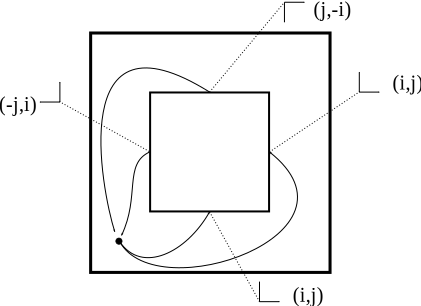
\includegraphics[width=2.5in]{monodromy.png}
\caption{Effect a nontrivial loop has on basis vectors $(i,j)\in\RR^2$.}
\label{fig:loop}
\end{figure}

\begin{lem}
$\varphi_2:\pi_1(\bGs)\rightarrow \mathrm{SO}(2,\ZZ)$ is the rotational monodromy representation of $\bGs$.
\begin{proof}
From Figure 4 it's clear that $c,d$ will rotate a unit vector by $\pm 90^\circ$ by parallel transport along their paths. These values are determined by the cone angles of the singularities they loop around. The parallel transport of a vector along $a$ or $b$ would be trivial since the outer edges they pass through are glued by translation.
\end{proof}
\end{lem}


\begin{lem}
Any element in $\text{Deck}(\varphi_1^*)$ acting on $T^1\bUs$ has a trivial effect on holonomy.
\begin{proof}
Since $\bGs=\bUs/\ZZ^2$, the deck group action lifts naturally to an action on their tangent vector spaces and unit tangent bundles via pushforward of deck transformations $f_h,f_v$ on the bundle maps. i.e. $T^1\bGs=T^1\bUs/\ZZ^2$. This effect must be trivial since $\varphi_1(a)\sim f_h$ and $\varphi_1(b)\sim f_v$, and both homotopy classes $a,b$ have trivial holonomy.  \\
How do $f_h,f_v$ parallel transport a vector?\\
Well if $\varphi_1([a])\cdot u_0=f_h(u_0)$, then for 
\end{proof}
\end{lem}



\begin{thm}
Let $m=\varphi_2\vert_{\pi_1(\bUs)}$. Then $m$ is the rotational monodromy map of $\bUs$.
\begin{proof}

\end{proof}
\end{thm}

\begin{cor}
Let $\alpha:[0,1]\rightarrow\bGs$ be a loop on $\bGs$ with trivial holonomy and $\tilde{\alpha}$ its lift to $\bUs$. Then $\tilde{\alpha}$ has trivial holonomy as well.
\begin{proof}

\end{proof}
\end{cor} 

\begin{Def}
Let $\bMs$ be the regular cover of $\bGs$ with fundamental group $\pi_1(\bMs)=\ker\varphi_2$.
\end{Def}
Showing that $\bMs$ is a degree four cover of $\bGs$ with trivial holonomy and deck group $\SO(2,\ZZ)$ follows immediately from its construction.
\begin{figure}[H]
\centering
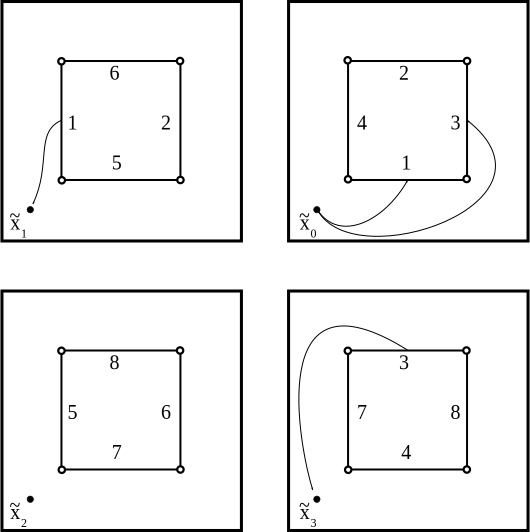
\includegraphics[width=3in]{monogroup.png}
\label{fig:arbitrarylift}
\caption{Lift of paths $c,d$ to $\bMs$ (\compav{RELABEL EDGES})}
\end{figure}


\subsection{A Four-Fold Cover}
We now take these covers we built to construct a third one that covers them all. This is a four-fold cover of $\bUs$ and a $\ZZ^2$ translation cover of $\bMs$. 
\begin{Def}
Let $\btUs$ be the cover of $\bUs$ with fundamental group $\pi_1(\btUs)=\ker\varphi_2\big\vert_{\pi_1(\bUs)}$.
\end{Def}

It follows that $\ker\varphi_1\big\vert_{\pi_1(\bMs)}=\ker\varphi_2\big\vert_{\pi_1(\bUs)}$ and that $\btUs$ is a cover of these two surfaces. Edge identifications are made on four copies of $\mathbf{P}$, possibly indexed by the finite component of the direct product $\mathbf{P}\times\ZZ/4\ZZ$. The Deck group of the covering map from $\btUs$ to $\bGs$ is the set $\ZZ^2\times \SO(2,\ZZ)$. Consider a loop on $\bUs$:

\begin{figure}[H]
\centering
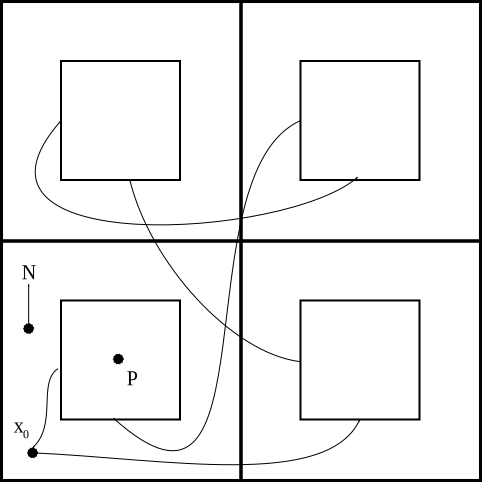
\includegraphics[width=2in]{overlay.png}
\end{figure}

\noindent If we lift this curve to $\btUs$ we can identify it with an element of the deck group, and check if its lift from $\bGs$ belongs to the kernel of both $\varphi_1$ and $\varphi_2$. Fix a direction on this surface pointing north that respects $\bUs$'s compass and rotate every plane by either $90^\circ,$ $180^\circ,$ or $270^\circ$ as the curve travels from one plane (copy of $\mathbf{P}$) to the next. Observe that it will not only close if the curve acts trivially on the holonomy of $\bUs$, but with this construction we can see that $\btUs$ is actually an infinite-type translation surface:

\begin{figure}[H]
\centering
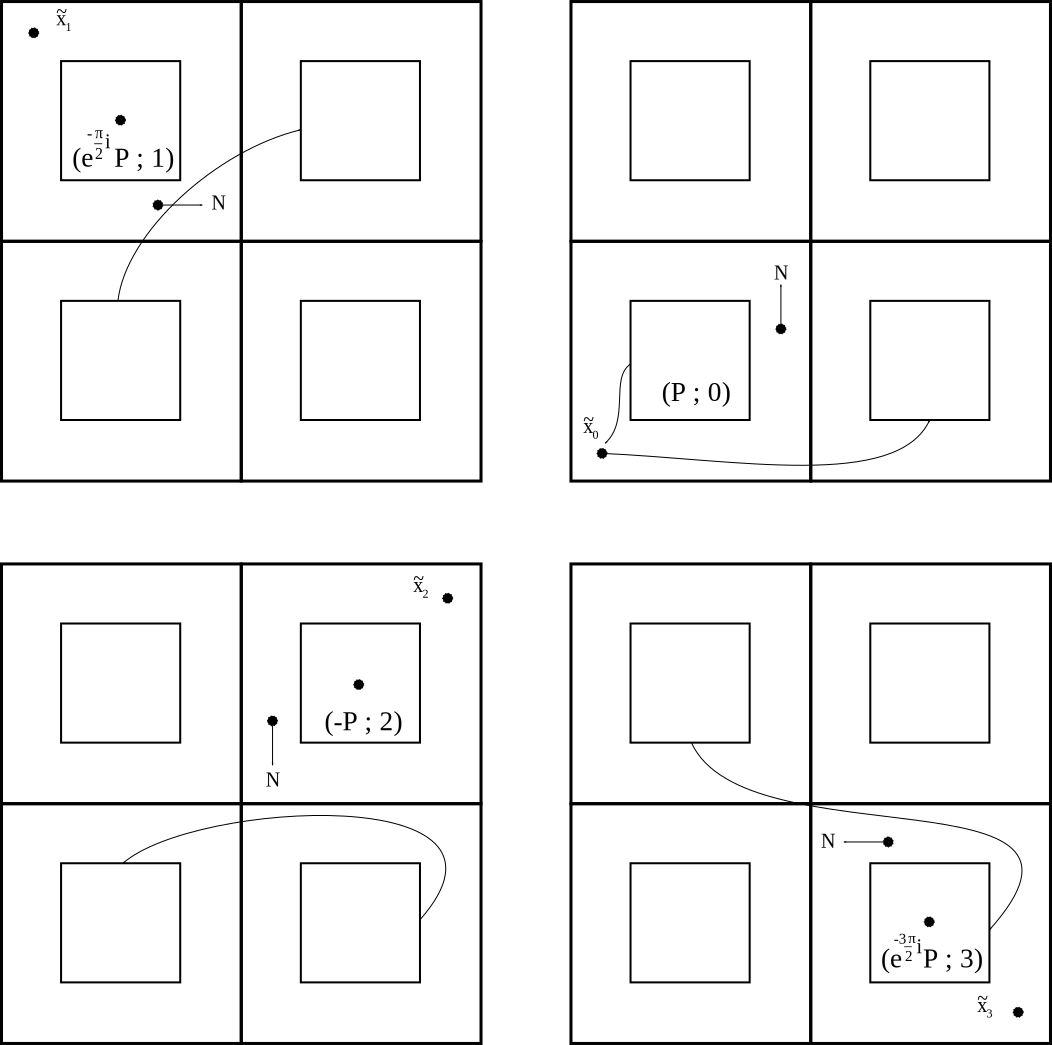
\includegraphics[width=3in]{coverdirection.png}
\caption{With $P\in 2\ZZ+2\ZZ i$.}
\end{figure}

\noindent 

\subsection{Geodesics on $\bUs$}
The key connection made between surfaces $\bUs$ and $\btUs$ is that geodesics on $\bUs$ and $\btUs$ behave identically. Unless stated otherwise, a \emph{geodesic} is a \emph{unit-speed} locally distance minimizing curve on a smooth topological surface as a function parameterized by an element in $\RR$. A \emph{geodesic segment} is a restriction of the geodesic to some closed interval in $\RR$. A geodesic has an initial trajectory defined at time 0, represented by a unit vector $v_0\in\RR^2$. If the vector can be scaled by $k\in\RR$ such that $kv_0\in\cS$, the geodesic has a \emph{rational} initial trajectory. For example, the following is a periodic geodesic on the surface with initial direction $kv_0\in\cO$:

\begin{figure}[H]
\centering
\includegraphics[width=4in.]{closed2.png}
\caption{Periodic geodesic path on $\bUs$ modeled with sage-flatsurf.}
\label{fig:complicated}
\end{figure}

We refer later to the following commuting diagram of branched covering maps and inclusion maps. It is meant to illustrate the relationship between all of these spaces.

\begin{equation}
\begin{tikzcd}
\arrow[two heads, bend left]{rrr}{f^\circ}[swap]{} \arrow[hook]{d}{pr_b} \btUs \arrow[two heads]{r}{r^\circ} & \bUs \arrow[hook]{d}{pr_c} \arrow[two heads]{r}{q^\circ} & \bGs \arrow[hook]{d}{pr_d} &\arrow[two heads]{l}{w^\circ} \bMs \arrow[hook]{d}{pr_a}  \\
\arrow[two heads, bend right]{rrr}{}[swap]{f} \btU \arrow[two heads]{r}{r} & \bU \arrow[two heads]{r}{q} & \bG & \arrow[two heads]{l}{w}\bM  \\
\end{tikzcd}
\label{eq:commute}
\end{equation}



Let $x_0\in G^\circ$ and fix $u_0\in\bUs$, an element in the fiber of the covering map. A \emph{geodesic} on $G^\circ$ is a closed unit-speed straight-line path given as $\eta:\RR\rightarrow\bGs$. The \emph{period}/\emph{length} of the geodesic is some strictly positive $b\in\RR$. Let $\eta|_{[0,b]}=\alpha:[0,b]\rightarrow\bGs$ be a closed geodesic segment on $\bGs$ with initial and terminal point $x_0$. Denote $\alpha$'s unique lift to $\bUs$ by $\gamma:[0,b]\rightarrow\bUs$, where $\gamma(0)=u_0$, and $\gamma(b)$ in the fiber over $x_0$. Fix a point $\utild\in\btUs$ in the fiber over $u_0$. We define the unique lift of $\gamma$ to be the curve $\tilde{\gamma}:[0,b]\rightarrow\btUs$ with $\tilde{\gamma}(0)=\utild$. Denote their homotopy class representatives by $[\alpha]$ and (if they exist) $[\gamma],~[\tilde{\gamma}]$.

The geodesic segment on $\bGs$ has the property that it returns to $x_0$ with a trivial effect on the holonomy of the curve. On the other hand, the lifted paths will close only if their homotopy classes belong in their fundamental groups, i.e. the kernel of homomorphisms $\varphi_1$, $\varphi_2|_{\ker\varphi_1}$. Otherwise they are mapped non-trivially to $\ZZ^2$ or $\ZZ^2\times\SO(2,\ZZ)$. Let $v_0\in\RR^2$ be a unit vector such that $\alpha's$ derivative is $v_0$ at times $0$ and $b$. The derivative of $\gamma$ is also $v_0$ at these times as per Corollary 1, as $\alpha$ is a geodesic with trivial holonomy. $\gamtild'$ are also $v_0$ at their endpoints.

The Deck group of the map $\btUs\rightarrow\bUs$ is $\SO(2,\ZZ)$. This deck group acts naturally on the tangent bundles via push-forward of rotational matrices. We obtain the identity $T^1\btUs/\SO(2,\ZZ)\cong T^1\bUs$. This action is \emph{non-trivial}. Essentially, this means that there are 4 choices of a vector on the four-fold cover given a vector $v_0$ on $\bUs$. The choice of vector does not matter in the case where we flow it along a geodesic path, as a geodesic must return to a point in the fiber of $u_0$ in the same direction. That is to say that no matter where we start by lifting this path, we will always end up on the same plane (copy of $\mathbf{P}$) that we started in. In the case where a geodesic is periodic on $\bUs$, it would return to the same point in the fiber of $u_0$ as well. For simplicity's sake we will just lift to the vector mod the identity matrix, and call it $v_0$ as well.

\begin{Def}
Let $\Phi_t:\RR\rightarrow\bUs$ be a unit-speed geodesic on the \emph{Necker cube surface} with $\Phi(0)=u_0$ and $\Phi'(0)=v_0$. \\Similarly, let $\tilde{\Phi}_t:\RR\rightarrow\btUs$ be a unit-speed geodesic on $\bUs$'s four-fold cover with $\phitild(0)=\utild$ and $\phitild'(0)=v_0$.
\end{Def}
Let $\varphi=\varphi_1\times\varphi_2:\pi_1(\bGs)\rightarrow \ZZ^2\times\SO(2,\ZZ)$ be given by $[g]\mapsto(\varphi_1([g]),\varphi_2([g]))$. $\varphi$ is a
product of group homomorphisms that takes a loop to 
\begin{thm}
Let $\delta=\varphi_1([\alpha])\in\ZZ^2$ be an element of $\Delta_{\varphi_1}$ and $\tilde{\delta}=\varphi([\alpha])\in\ZZ^2\times \SO(2,\ZZ)$ be an element of $\Delta_{\varphi}$. Then:\\
$\Phi(t+b)=\delta\cdot\Phi(t)$ for all $t\in\RR$, and 
$\phitild(t+b)=\tilde{\delta}\cdot\phitild(t)$ for all $t\in\RR$.
\end{thm}

\begin{cor}
The following are equivalent:
\begin{enumerate}
\item $\Phi$ is periodic.
\item $\phitild$ is periodic.
\item $\delta=(0,0)$.
\end{enumerate}
\end{cor}

\begin{cor}
The following are equivalent:
\begin{enumerate}
\item $\Phi$ is drift-periodic.
\item $\phitild$ is drift-periodic.
\item $\delta\neq(0,0)$.
\end{enumerate}
\end{cor}

These theorems essentially tell us that these types of geodesics behave identically on the Necker cube surface and its cover. Now we show that this is true for $\btUs$ and its metric completion, $\btU$.

\begin{equation}
\begin{tikzcd}
\arrow[hookrightarrow, bend left]{rrr}{f_*^\circ}[swap]{} \arrow[two heads]{d}{PR_b} \pi_1(\btUs) \arrow[hook]{r}{r_*^\circ} & \pi_1(\bUs) \arrow[two heads]{d}{PR_c} \arrow[hook]{r}{q_*^\circ} & \pi_1(\bGs) \arrow[two heads]{d}{PR_d} & \ar[hookrightarrow]{l}{}[swap]{w_*^\circ} \pi_1(\bMs) \arrow[two heads]{d}{PR_a} \\
\arrow[hookrightarrow, bend right]{rrr}{}[swap]{f_*}  \pi_1(\btU) \arrow[hook]{r}{r_*} & \pi_1(\bU) \arrow[hook]{r}{q_*} & \pi_1(\bG) & \ar[hookrightarrow]{l}{}[swap]{w_*} \pi_1(\bM)\\
\end{tikzcd}
\label{eq:homomorphism}
\end{equation}



\begin{Def}
Let $\tildphi:\RR\rightarrow\btU$ be a geodesic on the unpunctured four-fold surface such that $\tildphi(0)=\utild$ and $\tildphi'(0)=v_0$.
\end{Def}

\begin{thm}
$\tildphi$ is periodic if and only if $\phitild$ is periodic.\\
$\tildphi$ is drift-periodic if and only if $\phitild$ is drift-periodic.
\end{thm}

This follows readily from the fact that geodesics are undefined on cone singularities. A geodesic on $\btUs$ can be mapped bijectively to a geodesic on  $\btU$ and vice-a-versa.



\subsection{Translation Surface}
Consider the projection $\btU\rightarrow\mathbf{M}$ onto a quotient of the surface under its translational symmetries of each plane (see Fig 6). What we obtain is a genus 5 finite translation surface $\bM-$ also a branched cover of $\bG$. $\bMs$ was obtained as a cover of $\bGs$ from the rotational monodromy map on $\pi_1(\bGs)$, so $\bM$ is just its metric completion by reintroducing these vertices. There are four cone singularities on this surface, as opposed to the three on $\bG$, each of cone angle $6\pi$. Keeping track of $\btU$'s compass pointing \emph{true} north, the individual sections of $\bM$, labeled $I,II,III,$ and $IV$, are rotated in such a way to \emph{trivialize} \emph{holonomy} on arbitrary paths (Fig 8). Observe that $\bM$ is really a square-tiled/origami surface constructed out of unit squares (Fig 9).

\begin{figure}[H]
\centering
\includesvg[width=2.6in]{mtildabw}
\caption{Compact translation surface, $\mathbf{M}$ with edges and cone singularities (1,2,3,4) identified. The Roman numerals are meant to identify every ``copy" of $\bG$ with a direction differing from $v_0$ by rotation of some element in $\SO(2,\ZZ)$. The individual copies are then rotated so every edge is identified by translation.}
\label{fig:mtilda}
\end{figure}

\begin{figure}[H]
\centering
\includesvg[width=3.4in]{mtildastaircasebw}
\caption{The staircase surface with directional planes and vertices identified. All edges are paired by translation. Two adjacent squares have opposite edges (A-M) identified. The top edge of the bottom-left square is glued to the bottom edge of the top-right square (both labeled I). Likewise, the bottom edge of the bottom-left square is identified with the top edge of the top-right square.}
\label{fig:staircase}
\end{figure}

\noindent We recall some basic properties of $\ZZ^2$ covers of translation surfaces as they apply to $\bM$. 

The set of all orientation preserving affine diffeomorphisms of $\bM$ form the group $\text{Aff}^+(\bM)$. The \emph{Veech group} of $\bM$ is the image of $\text{Aff}^+(\bM)$ in $SL(2,\RR)$ under the derivative map, $D:\text{Aff}^+(\bM)\rightarrow SL(2,\RR)$. We denote this group $V(\bM)$. It is a well-known fact that square-tiled surfaces like $\bM$ are \emph{Veech} and have Veech groups of finite index in $\SL(2,\ZZ)$ [Gutkin-Judge]. We use $V(M)$ and the $\text{Aff}^+(\bM)$-induced automorphism group, $\text{Aut}(\pi_1(\bM))$, as they act on geodesics and their homotopy classes. When we reconstructed $\bM$ as a staircase, we kept track of the outer edges of the surface that were identified with one another under the projection map defined on $\btU$. These now form cylinder core curves that are divided into homology classes $u,v,z$ (Fig 10). We denote the \emph{set of all core curve homology classes} by $\Gamma=\{[\gamma_i]~:~0\leq i \leq 11\}$.

\begin{figure}[H]
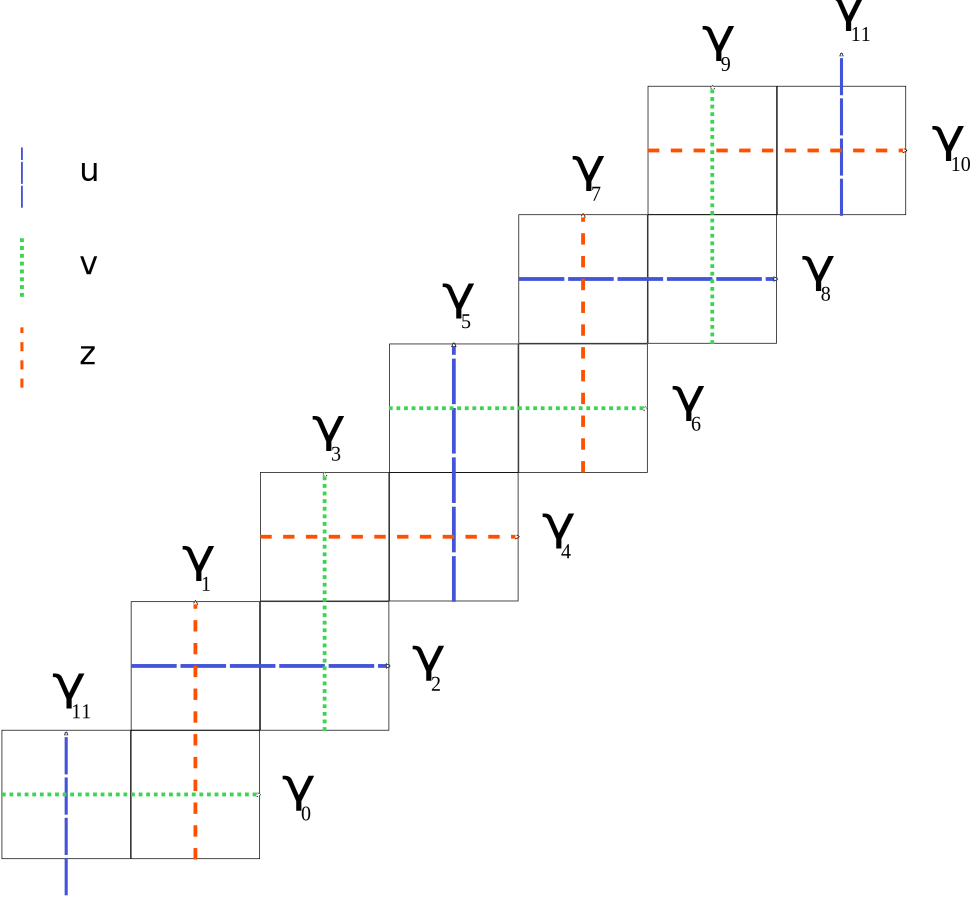
\includegraphics[width=3in]{homologyclass.png}
\centering
\caption{$\bM$'s cylinder core curves with u,v, and z homology class labels.}
\label{fig:homology}
\end{figure}

We assign $u,v$ classes integer weights according to what translational effect \emph{crossing} the curve would have on a loop being lifted to the cover $\btU$. For example, a path crossing $[\gamma_0]$ and making a positive angle relative to the direction $\gamma_0$ is moving in (right) corresponds to moving ``up" once on $\btU$ from whatever section in the fiber of $\bM$ under the projection map on $\btU$ the lifted path might have belonged to prior to intersecting with $\gamma_0$. We would then assign to $[\gamma_0]$ the weight $(0,+1)\in\ZZ^2$. Crossing a curve in the $z$ class really does not take a path to another element in the fiber.

\begin{Def}
Algebraic intersection number is a non-degenerate bilinear form:
\begin{align*}
i:H_1(\bM,\QQ)\times H_1(\bM,\QQ)\rightarrow\ZZ.
\end{align*}
For $[\alpha],[\beta]\in H_1(\mathbf{M},\QQ)$, $i([\alpha],[\beta])$ returns the signed intersection number of two homology classes. We say a crossing at the moment of intersection is positive (+1) if $\beta$ makes a positive angle relative to the direction $\alpha$ is traveling in. A crossing is negative (-1) if $\beta$ makes a negative angle relative to $\alpha$.
\end{Def}

By observation, these signed weights are determined as follows:

\begin{Def}
The homology classes $u,v,z$ are given as the following weighted sums of elements of $\Gamma$:
\begin{align*}
u &= -[\gamma_2] +[\gamma_5] + [\gamma_8] - [\gamma_{11}],\\
v &= +[\gamma_0] -[\gamma_3] -[\gamma_6] +[\gamma_9],\\
z &= +[\gamma_1] +[\gamma_4]-[\gamma_7]-[\gamma_{10}].
\end{align*}
\end{Def}

\begin{rem}
To be precise, we can think of $\btU$ as a $\ZZ^2$ cover only because we take 8 homology classes and apply the necessary transformations (change of sign) that agree with the deck group of the covering map from $\btUs$ to $\bGs$, $\ZZ^2\times\SO(2,\ZZ)$. Note that this group is isomorphic to $\ZZ^8$.
\end{rem}

By constructing a $12\times12$ intersection matrix and calculating its rank (rank=10), we can see that $\Gamma$ does span $H_1(\bM,\QQ)\cong\ZZ^{10}$ and does not need every cylinder curve. Certain relations can be discerned, such as $u+v=z$, to reduce the set to ten elements but the indexing scheme of $\Gamma$ here is far easier to work with, being in agreement with $\bM$'s cylinder decomposition in vertical and horizontal directions. This comes at the cost of the vector space being overdetermined and not having a coordinate basis, but it is not necessary to have one here.

\begin{Def}
Fix $m_0\in\bM$ and let $\mtild\in\btU$ be a point in the fiber of $m_0$. Let $\Omega_{u,v}:\pi_1(\bM)\rightarrow \ZZ^2$ be the homomorphism relating an $m_0$-based loop's intersection number with homology classes $u,v$ to the terminating point of its lifted path based at $\mtild$ on $\btU$. If $\beta$ is such a loop, then 
\begin{align*}
\Omega_{u,v}([\beta])=(i(u,[\beta]),~i(v,[\beta]))
\end{align*}
\end{Def}

\begin{thm}
The cover $\btU$ has first fundamental group $\ker\Omega_{u,v}$.
\begin{proof}
\end{proof}
\end{thm}

\subsection{Induced Automorphisms of $H_1(\bM,\QQ)$}
We look at some important automorphisms induced by Affine maps on $\bM$. Observe that $\bM$ has a uniform cylinder decomposition in both horizontal and vertical directions (Fig 15). We define the \emph{modulus}, $\mu$, of a cylinder to be the ratio of the cylinder's width to its circumference, $\frac{w}{c}$. The $\emph{Dehn-twist}$ of a cylinder is an affine diffeomorphism that skews the cylinder and preserves edges and vertices.

\begin{figure}[H]
\centering
\includesvg[width=3in]{cylinderskew}
\label{fig:skew}
\caption{Dehn-twist of a cylinder in $\bM$'s cylinder decomposition.}
\end{figure}

Such a map has derivative $\left[~\begin{matrix}1 && \pm\mu^{-1}\\0 && 1\end{matrix}~\right]$. On $\bM$ all cylinders in both vertical and horizontal decompositions have moduli $\mu=\frac{1}{2}$. These give up global diffeomorphisms as $\emph{multi-twists}$ of $\bM$ with the same derivative. [cite] 

\begin{Def}
We define the global affine diffeomorphisms of $\text{Aff}^+(\bM)$ obtained as \textbf{multi-twists of the surface in horizontal and vertical directions} $\psi_h$ and $\psi_v$, respectively.
\end{Def}

The twists $\psi_h$ and $\psi_v$ under derivative map $D$ are mapped to the same matrices as the Dehn-twists. i.e.
\begin{align*}
D(\psi_h)=\psi_h'=\left[ \hspace{1mm} \begin{matrix}
				1 &   2\\
				0 & 1
			\end{matrix}\hspace{1mm}\right] \hspace{0.5in}
			D(\psi_v)=\psi_v'=\left[ \hspace{1mm} \begin{matrix}
							1 & 0\\
							 2 & 1
						\end{matrix}\hspace{1mm}\right]
\end{align*}

These are parabolic elements of $V(\bM)$ that generate a free group of rank 2. [cite].
\begin{Def}
Let $\XX$ be the generated parabolic subgroup of $\text{Aff}^+(\bM)$, where $\XX=\<\psi_h,\psi_v \>$.
\end{Def}

The image of this group under $D$ is itself a subgroup of $V(\bM)$ and denoted $D(\XX)=\XX'=\<\psi_h',\psi_v' \>$ as in page 2. When skewing the surface and piecing it back together under $\psi_h$ or $\psi_v$, the cylinder curves intersect each other in pairs:

\begin{figure}[H]
\centering
\includesvg[width=2in]{skew}
\end{figure}

By skewing in the horizontal direction, $\psi_h$ preserves the even indexed cylinder curves, but the odd indexed vertical curves $\gamma_i$ intersect the two horizontal curves (positive intersection), $\gamma_{i-1}$ and $\gamma_{i+1}$. A similar observation can be made from applying $\psi_v$, where the vertical curves are preserved but the horizontal curves intersect with adjacent vertical curves (negative intersection). Let $i\in\ZZ/12\ZZ$. Then the following formulas hold for $\psi_h$ and $\psi_v$'s counterparts in $\Aut(H_1(\bM,\QQ))$ raised to $k\in\ZZ\backslash\{0\}$:

\begin{align*}
\psi^{*k}_h([\gamma_i])=&[\gamma_i] + \frac{k}{2}(1-(-1)^i)([\gamma_{i-1}]+[\gamma_{i+1}])\\
\psi^{*k}_v([\gamma_i])=&[\gamma_i] - \frac{k}{2}(1+(-1)^i)([\gamma_{i-1}]+[\gamma_{i+1}])\\
\end{align*}

If $k=0$, then it's just the identity. We generate the group $\XX^*=\<\psi^{*}_h,\psi^{*}_v \>$. There are no relations between its generators since $i$, being even or odd, has one automorphism act trivially while the other acts non-trivially. Therefore this group is also a free group of rank 2. All of our related groups are free groups, so we have that $\XX^*\cong\XX'\cong\XX$. 


Let $\tau\in\XX$. Let $D(\tau)=\tau'\in\XX'$ and $\tau^*\in\XX^*$ be isomorphic elements in their respective groups. We say $\tau=\prod_{j=0}^{n}\psi_h^{k_j}\circ\psi_v^{m_j}$ is a word in $\XX$ as a finite left concatenated product of multi-twist pairs with $k_j,m_j\in\ZZ$. Let $\psi_j=\psi_h^{k_j}\circ\psi_v^{m_j}$ be the $j^{th}$ multi-twist pair. Since $\tau',\tau^*$ are isomorphic, we can use their expressions interchangeably. \\\\
The $j^{th}$ automorphism pair is an element $\psi_j^*\in\Aut(H_1(\bM,\QQ))$ and can be expressed as 

\begin{align*}
\psi_j^*([\gamma_i])=&[\gamma_i]+\frac{k_j(1-(-1)^i)}{2}([\gamma_{i-1}]+[\gamma_{i+1}])\\&-\frac{m_j(1+(-1)^i)}{2}(k_j(2[\gamma_i]+[\gamma_{i-2}]+[\gamma_{i+2}]) +[\gamma_{i-1}]+[\gamma_{i+1}]).
\end{align*}

\noindent Similarly,

\begin{align*}
\psi_j'=\left[ \hspace{1mm} \begin{matrix}
				1 &   2\\
				0 & 1
			\end{matrix}\hspace{1mm}\right]^{k_j}\left[ \hspace{1mm} \begin{matrix}
							1 &   0\\
							2 & 1
						\end{matrix}\hspace{1mm}\right]^{m_j}=\left[ \hspace{1mm} \begin{matrix}
										1+4m_jk_j &   2k_j\\
										2m_j & 1
									\end{matrix}\hspace{1mm}\right]
\end{align*}


\noindent Let $\sum\Gamma=\sum_{i=0}^{11}[\gamma_i]$, and denote the odd and even indexed sums of core curves $\sum\Gamma_o$ and $\sum\Gamma_e$, respectively. We look at three kinds of closed geodesic segments on $\bM$ and don't consider initial/terminal points for the time being. These are the geodesics in directions $\theta=0,\frac{\pi}{2},$ and $\frac{\pi}{4}$. The aim is to show that these linear automorphisms take $\sum\Gamma\mapsto c_1\sum\Gamma_e+c_2\sum\Gamma_o$ and an individual $[\gamma_i]$ to an element that maps non-trivially to $\ZZ^2$ under $\Omega_{u,v}$. \\



\noindent Let $\chi$ be the geodesic segment in direction $\theta=\frac{\pi}{4}$ that runs up the staircase intersecting every $\gamma_i$ exactly once. Denote its homotopy class by $[\chi]$. Observe from Figure 10 that $\chi$ is homologous to $\frac{1}{2}\sum\Gamma$, a curve that climbs up the staircase. When lifted to $\btU$ and projected onto $\bUs$, this is a closed segment on the Necker cube surface (Fig 1).


\begin{lem}
$\Omega_{u,v}([\chi])=(0,0).$
\begin{proof}
Observe that $\Omega_{u,v}([\chi])=\Omega_{u,v}(\frac{1}{2}\sum\Gamma)=\frac{1}{2}(i(u,\sum\Gamma),i(v,\sum\Gamma)).$ Since only adjacent curves intersect, $i(u,\sum\Gamma)=i(-[\gamma_2],[\gamma_{1}]+[\gamma_{3}]) +i([\gamma_5],[\gamma_{4}]+[\gamma_{6}]) + i([\gamma_8],[\gamma_{7}]+[\gamma_{9}]) - i([\gamma_{11}],[\gamma_{10}]+[\gamma_{0}])=-2+(-2)+2-(-2)=0$.\\
Similarly, $i(u,\sum\Gamma)=i([\gamma_0],[\gamma_{11}]+[\gamma_{1}]) -i([\gamma_3],[\gamma_{2}]+[\gamma_{4}]) -i([\gamma_6],[\gamma_{5}]+[\gamma_{7}]) +i([\gamma_9],[\gamma_{8}]+[\gamma_{10}])=2-(-2)-2+(-2)=0$. Therefore, $\Omega_{u,v}([\chi])=(0,0)$.
\end{proof}
\end{lem}

Thus $\chi$ lifts to a closed geodesic segment on $\btU$. Now any geodesic segment in the orbit of $\chi$ under $\XX$ is taken into consideration, and we see why taking sums of gamma curves to sums of even and odd curves are so important.

\begin{lem}
Let $\tau$ be as above. If $\alpha=\tau(\chi)$ is a closed geodesic segment on $\bM$, then $[\alpha]=\frac{1}{2}(c_1\sum_e+c_2\sum_o)$ for $c_1,c_2\in\ZZ$.
\begin{proof}(By Induction on $\psi^*_j\in\XX^*$).\\
Consider $\psi_0(\chi)$.\\
$[\psi_0(\chi)]=\psi_0^*[\chi]=\frac{1}{2}\psi_0^*(\sum\Gamma)=\frac{1}{2}\psi_0^*(\sum\Gamma_e+\sum\Gamma_o)=\frac{1}{2}(\psi_0^*(\sum\Gamma_e)+\psi_0^*(\sum\Gamma_o))$. Now\\ $\psi_0^*(\sum\Gamma_e)=\sum_{i=0}^{11}\psi_0^*([\gamma_{2i}])=\sum_{i=0}^{11}( [\gamma_{2i}]-2m_0k_0[\gamma_{2i}]-m_0k_0[\gamma_{2i-2}] $\\$ -m_0k_0[\gamma_{2i+2}]-m_0[\gamma_{2i+1}]-m_0[\gamma_{2i-1}] )=(1-4m_0k_0)\sum\Gamma_e+(-2m_0)\sum\Gamma_o$.\\
Now\\ $\psi_0^*(\sum\Gamma_o)=\sum_{i=0}^{11}\psi_0([\gamma_{2i+1}])=\sum_{i=0}^{11}([\gamma_{2i+1}] +k_0([\gamma_{2i}]+[\gamma_{2i+2}]))=\sum\Gamma_o+2k_0\sum\Gamma_e$.\\
And so $\frac{1}{2}\psi_0^*(\sum\Gamma)=\frac{1}{2}((1+2k_0-4k_0j_0)\sum\Gamma_e +(1-2m_0)\sum\Gamma_o )$.\\\\
Induction: Suppose $\frac{1}{2}\psi^*_j(\sum\Gamma)=c_1\sum\Gamma_e+c_2\sum\Gamma_o$.\\
Then $\psi^*_{j+1}(\psi^*_{j}(\sum\Gamma))=c_1\psi^*_{j+1}(\sum\Gamma_e)+c_2\psi^*_{j+1}(\sum\Gamma_o)=\\
c_1((1-4m_{j+1}k_{j+1})\sum\Gamma_e+(-2m_{j+1})\sum\Gamma_o)+c_2(\sum\Gamma_o+2k_{j+1}\sum\Gamma_e)=\\
(c_1(1-4m_{j+1}k_{j+1}) + 2k_{j+1}c_2)\sum\Gamma_e+(-2m_{j+1}c_1+c_2)\sum\Gamma_o$.\\
Therefore, $[\alpha]=\frac{1}{2}(c_1'\sum_e+c_2'\sum_o)$

\end{proof}
\end{lem}

\begin{thm}
Let $\tau$ be as above. Suppose $\alpha=\tau(\chi)$. Then $\Omega_{u,v}([\alpha])=(0,0)$. 
\begin{proof}
$\Omega_{u,v}([\alpha])=\Omega_{u,v}([\tau(\chi)])=\Omega_{u,v}(\tau^{*}([\chi]))=\frac{1}{2}(i(u,\tau^*(\sum\Gamma)) i(v,\tau^*(\sum\Gamma))$.\\
First consider $i(u,\tau^*(\sum\Gamma)=c_1 i(u,\sum
\Gamma_e)+c_2 i(u,\sum\Gamma_o)$ by previous Lemma. $\\= c_1(i([\gamma_5],[\gamma_{4}]+[\gamma_6]) - i([\gamma_{11}],[\gamma_{10}]+[\gamma_{0}]))\\+c_2(-i([\gamma_2],[\gamma_{1}]+[\gamma_{3}]) + i([\gamma_8],[\gamma_{7}]+[\gamma_{9}]) )=\\c_1((-2)-(-2))+c_2(-2+ 2 )=0\\$
The same holds for $i(v,\tau^*(\sum\Gamma)).$\\
$\therefore \Omega_{u,v}([\alpha])=(0,0)$.
\end{proof}
\end{thm}

Now we know that $\chi$ serves as something of a basis for a class of lifted closed segments. To show that these are the only (rational direction) segments that lift to closed segments on $\btU$, we look at the orbit of segments in directions $\theta=0,$ and $\frac{\pi}{2}$ that are homologous to some $\gamma_i$.

\begin{lem}
$\Omega_{u,v}([\gamma_i])\neq (0,0)$.
\begin{proof}
Every curve, $\gamma_i$, intersects exactly one adjacent index curve that is an element of exactly one of either $u$ or $v$, or with one of both $u$ \emph{and} $v$. Therefore, it is always taken to some non-trivial element of $\ZZ^2$ under $\Omega_{u,v}$.
\end{proof}
\end{lem}

\begin{thm}
Suppose $\beta=g(\gamma_i)$. Then $\Omega_{u,v}([\beta])\neq (0,0)$.
\begin{proof}
$g^*([\gamma_i])=[\gamma_i]+C$.
If $i(u,g^*([\gamma_i]))=i(u,[\gamma_i]+C)=i(u,[\gamma_i])+i(u,C)=0$, then 
\end{proof}
\end{thm}


\section{Proof of Main Theorem}
Knowing that geodesic segments in the orbit of $\chi$ and an element of $\Gamma$ are mapped either trivially or non-trivially, we use the fact that $\XX\cong\XX'$ to show that every rational direction is attainable from these elements. Recall that $\frac{1}{k}(x,y)\in S=\cO\cup \cE$ is a unit vector, and $(x,y)$ is an element of $\ZZ^2$ with $x,y$ relatively prime. Further partition $\cE$ into sets $\cE_1$ and $\cE_2$, where integer pairs $\frac{1}{k}(x,y)\in\cE$ are in $\cE_1$ if $x$ is odd or in $\cE_2$ if $x$ is even. These are disjoint since $x$ and $y$ cannot both be even or odd at the same time. Let $\XX'$ act on $\cS$ by linear transformations on $\ZZ^2$. We make use of Bezout's identity frequently. That is for any relatively prime $x,y$ there exist $m,n\in\ZZ$ such that $mx+ny=1~(*)$.

\subsection{Orbit of Rational Directions}

\begin{lem}
$\XX'=\ker p$ where $p:M\mapsto M~(mod~2)$. [cite]
\end{lem}

\begin{lem}
$\XX'$ acts faithfully and transitively on $\cO$.
\begin{proof}
Let $v_0=\begin{pmatrix}x \\ y\end{pmatrix}\in\cO$, where $x,y$ are both odd and relatively prime integers. Let $M=\begin{pmatrix}a & b \\ c & d
\end{pmatrix}\in\XX'$. Let $u=\begin{pmatrix}1 \\ 1 \end{pmatrix}\in\cO$. It follows from the previous lemma that this action is faithful since $ax+by$ and $cx+dy$ cannot sum up to an element in $\cE$, as $a,d$ are odd and $b,c$ are even. We show that there is a matrix $M$ such that $Mu=v_0$, i.e. $a+b=x$ and $c+d=y$. We know $\det M=ad-bc=1$ and from $(*)$ that there exist $m,n\in\ZZ$ such that $1=mx+ny$. Let $a=(x-b)$, $b=n(xy-1)$, $c=m(xy-1)$, and $d=(y-c)$. Then
\begin{align*}
\det M&=(x-n(xy-1))(y-m(xy-1))-n(xy-1)m(xy-1)\\
&=xy-mx(xy-1)-ny(xy-1)+mn(xy-1)^2-mn(xy-1)^2\\
&=xy-x^2my-y^2nx+(mx+ny)=xy-xy(mx+ny)+1\\
&=xy-xy+1=1.
\end{align*}
Therefore $M\in\SL(2,\ZZ)$. Now its simple to show that $a+b=(x-b)+b=x$ and $c+d=c+(y-c)=y$. Now $b=n(xy-1)$ and $c=m(xy-1)$ are even since $xy-1$ is even, and so $a=x-b$ and $d=y-c$ are odd. Hence, $M\in\ker p$ and $Mu=v_0$. $M$ is invertible, so $M^{-1}v_0=u.$ Apply the same argument for some other $v_0'\in\cO$, and obtain that $N^{-1}v_0'=u.$ We conclude then that $NM^{-1}v_0=v_0'$ for any $v_0,v_0'\in\cO$.
\end{proof}
\end{lem}

\begin{lem}
$\XX'$ acts faithfully and transitively on $\cE_1$ and $\cE_2$.
\begin{proof}
Likewise, faithfulness follows immediately from Lemma [something]. Let $v_0=\begin{pmatrix}x \\ y\end{pmatrix}\in\cE$, where $x,y$ are both odd and relatively prime integers. Let $M=\begin{pmatrix}a & b \\ c & d
\end{pmatrix}\in\XX'$. Let $u_1=\begin{pmatrix}1 \\ 0 \end{pmatrix}\in\cE_1$ and $u_1=\begin{pmatrix}0 \\ 1 \end{pmatrix}\in\cE_2$.\\\\
Case I: $v_0\in cE_1$. Then let $a=x$, $b=-n$, $c=y$, and $d=m$, where $mx+ny=1$ by $(*)$. Then
\begin{align*}
\det M &= ad-bc=xm-(-ny)=mx+ny=1.
\end{align*}
Hence, $Mu_1=v_0$. Repeating this argument for $u_1'\in \cE_1$, we get that $Nu_1'=v_0$ and so $u_1'=N^{-1}Mu_1$.\\\\
Case II: $v_0\in cE_1$. The proof for this is analogous to Case I.
\end{proof}
\end{lem}

\subsection{Directions and Orbit of Geodesic}
We can always pullback a geodesic segment on $\bM$ by associating with it a vector in $\RR^2$ because it is a translation surface. Let $\hol:\pi_1(\bM)\rightarrow\RR^2$ be the translational holonomy map that takes a closed path to its endpoint in local coordinates on the plane starting from the origin. For example, for the slope one geodesic segment $\chi$, $\hol([\chi])=(6,6)$.

\begin{lem}
Let $\alpha=\tau(\chi)$ be a geodesic segment in the orbit of $\chi$ under $\XX$. Then $\hol([\alpha])=\tau'\cdot\hol([\chi])$ with $\tau'=D(\tau)$. 
\end{lem}

\begin{lem}
Let $\beta_h=\tau(\gamma_0)$ and $\beta_v=\tau(\gamma_{11})$ be geodesic segments in the orbit of $\gamma_0$, $\gamma_{11}$ under $\XX$. Then $\hol([\beta_h])=\tau'\cdot\hol([\gamma_0])$ and $ \hol([\beta_v])=\tau'\cdot\hol([\gamma_{11}])$ with $\tau'=D(\tau)$. 
\end{lem}

\begin{Def}
Let $\phi_t^\theta:\RR\rightarrow\bM$ be a unit-speed geodesic with base point $m_0$ in direction $\theta\in \RR/2\pi\ZZ$. Denote $\phi$'s geodesic lift onto $\btU$ $\tildphi_t^\theta:\RR\rightarrow\btU$, where $\tildphi^\theta(0)=\mtild$ is a fixed base point in the fiber over $m_0$ under the projection map. Let $v_\theta=(\cos\theta,\sin\theta)\in\RR^2$ be a unit-vector in direction $\theta$.
\end{Def}

\begin{thm}
Let $\tildphi_t^\theta$ be a geodesic on $\btU$. Suppose there is some $k\in\RR$ such that $kv_\theta\in\cS$. Then $\tildphi_t^\theta$ is periodic with period $T=6\tau'\cdot (1,1)$ for some $\tau'\in\XX'$ if and only if $kv_\theta\in\cO$.
\end{thm}


\begin{thm}
Let $\tildphi_t^\theta$ be a geodesic on $\btU$. Suppose there is some $k\in\RR$ such that $kv_\theta\in\cS$. Then $\tildphi_t^\theta$ is drift-periodic with period $T=2\tau'\cdot (1,0)$ or $2\tau'\cdot(0,1)$ for some $\tau'\in\XX'$ if and only if $kv_\theta\in\cE$.
\end{thm}

\subsection{Embedding the Necker Cube Surface in $\RR^3$}
this section is about the map from $\RR^2$ to $\RR^3$ that embeds the cube surface. We finally show the relationship between euclidean distances in its embedding and $\Delta_{\varphi_1}$

\subsection{Dynamical Classification Theorem}
\begin{thm*}
(Dynamical Classification of Geodesics on the Necker Cube Surface) \\Let $\Phi_t:\RR\rightarrow\bUs$ be a non-singular unit-speed geodesic on the Necker cube surface such that $\Phi(0)=u_0$ and $\Phi'(0)=v\in\RR^3$, isometric to $v_0\in\RR^2$. Let $\overline{u}_t\in\RR^3$ be $\Phi_t$'s coordinate in $\bUs$'s ambient space at time $t$. Let $k\in\RR$ such that $kv_0\in\cS$. Then the following is true:
\begin{enumerate}[label=(\roman*)]
\item $\Phi$ is periodic if $kv_0\in\cO$.
\item Suppose $\Phi$ is periodic. If $M (kv_0)=(1,1)$ then $\Phi$ has period $T=6\sqrt{2}||kv_0||$.
\item $\Phi$ is drift-periodic if $kv_0\in\cE$. 
\item Suppose $\Phi$ is drift-periodic. If $M (kv_0)=(1,0)$ or $M (kv_0)=(0,1)$ then $\Phi$ has period $T=2||kv_0||$, and $d_E(\overline{u}_t,\overline{u}_{t+T})=||kv_0||\sqrt{2}$.
\end{enumerate}
\end{thm*}

\newpage
~
\newpage

\begin{lem}
$\XX'$ acts faithfully and transitively on integer pairs in $\cO$, partitions $\cE$ into two sets and acts faithfully and transitively on them, and acts faithfully on $\cS$.
\begin{proof}
Let $v=kv_0=\begin{pmatrix}x \\ y\end{pmatrix}\in\cS$ with $||v_0||=1$ and $k\in\RR$, and let $A=\begin{pmatrix}a & b \\ c & d
\end{pmatrix}\in\XX'$. The kernel of the homomorphism $SL(2, \ZZ)\rightarrow \SL(2,\ZZ/2\ZZ)$ that maps a matrix to its $(mod~2)$ equivalent is precisely $\XX'$ since it maps the generators trivially. [quote this paper for the proof of this maybe? http://www.fysik.su.se/~ingemar/SL2.pdf ]\\
$x,y$ are relatively prime, so Bezout's identity states there exist $m,n\in\ZZ$ such that $mx+ny=1~(*)$. It's obvious that this action is faithful on the sets since the stabilizer of any vector in $\RR^2$ is trivial. Suppose $v\in\cO$. Consider the orbit of $\begin{pmatrix}1 \\1 \end{pmatrix}$. Then there is some matrix $A\in\XX'$ such that $A\begin{pmatrix}1\\1\end{pmatrix}=v$. Since $A\in\SL(2,\ZZ)$, $\det A = ad-bc=1$. Obtain from $1=(x-b)(y-c)-bc=xy-xc-by$ that $xy-1=xc+by$. From $(*)$ we see that $xy-1=x(u(xy-1))+y(v(xy-1))$. Let $c=u(xy-1)$ and $b=v(xy-1)$. Since $xy-1$ is even, $c,b$ are even. It follows then that $a=x-b$ and $d=y-c$ are odd. Therefore $A\in \XX'$ and the action is transitive on $\cO$. If $v\in\cE$, then either $x$ or $y$ is even. In either case this would mean that either $a$ or $d$ is even, which would mean $A\notin\XX'$, a contradiction.\\
Now consider the orbit of $\begin{pmatrix}1\\0\end{pmatrix}$. Left multiplying by $A$ would mean $a=x$ and $c=y$. Split $\cE$ into sets $\cE_1=\{(x,y)\in\cE :x\in2\ZZ,~y\in(2\ZZ+1) \}$ and $\cE_2=\{(x,y)\in\cE:x\in(2\ZZ+1),~y\in2\ZZ \}$. Since $\det A=1=da-bc=dx-by=mx+ny$, we have that $d=m$ and $b=-n$. We rule out when $v\in\cO,\cE_1$ since $c\neq 0 (\mod 2)$ in those cases. Consider $v\in\cE_2$. Then $x$ is odd and $y$ is even. $d$ must be odd since $mx+ny=1$ and $y$ is even. And $b$ must be even since $ad-bc=1$\\
\compav{finish this and say the proof for $\cE_1$ is analogous.}

\end{proof}
\end{lem}

\begin{Def}
Let $\phi_t^\theta:\RR\rightarrow\bM$ be a non-singular unit-speed geodesic on $\bM$ in direction $\theta$ based at $y_0$.
\end{Def}

Every rational direction geodesic closes so $\:\pi_1(\bM)\rightarrow\RR^2$ is well-defined for $\theta$ rational. Let $\alpha:[0,L]\rightarrow\bM$ be a closed geodesic segment of length L with image $\alpha([0,L])=\phi(\RR)$. Let $v_0=(\cos\theta,\sin\theta)$.

\begin{thm}
content...
\end{thm}

\subsection{empty}
\noindent Consider the following families of unit squares in $\RR^3$:\\
\vspace{0.2in}
\begin{tabular}{p{10cm}c}
\begin{align*}
\mathbf{A}_{m,n,p} = [m, m+1]\times[n,n+1]\times\{p\}, 
\\\mathbf{B}_{m,n,p} = \{m+1\}\times[n,n+1]\times[p-1,p],
\\\mathbf{C}_{m,n,p}= [m,m+1]\times\{n+1\}\times[p-1,p].
\end{align*}
&
\shiftleft{0.8in}{\raisebox{-1in}{
\includegraphics[scale=1]{label.png}}}
\end{tabular}


\begin{figure}[H]
\centering
\includesvg[width=1in]{cubesxyzcut}
\caption{A section of $\mathbf{S}$}
\end{figure}

\subsection{Flattening $\mathbf{S}$}
At the moment it is difficult to describe how the parallel transport of a vector tangent to the surface along an arbitrary path on the surface acts on the vector in $\RR^3$. To simplify this problem we take $\mathbf{S}$ to an isometric variant embedded in $\RR^2$ by piecewise linear transformations on the sets 
\begin{align*}
\mathbf{A}=\bigcup\big{\{}\mathbf{A}_{m,n,p}: m+n+p=0\big{\}},
\\\mathbf{B}=\bigcup\big{\{}\mathbf{B}_{m,n,p}: m+n+p=0\big{\}},
\\\mathbf{C}=\bigcup\big{\{}\mathbf{C}_{m,n,p}: m+n+p=0\big{\}}.
\end{align*}

\begin{Def}
Let $\Psi:s^*(\mathbf{S})\rightarrow\RR^3$ be given as
\begin{equation}
\Psi\left[\begin{array}{c}
	x\\y\\z
\end{array}\right] 
= 
\begin{cases}
	\left[ \hspace{2mm} \begin{matrix}
		1 & 0 & 0 \\
		0 & 1 & 0 \\
		0 & 0 & 1
	\end{matrix}\hspace{3mm}\right]

	\left[\begin{array}{c}
	x - \left\lfloor x \right\rfloor
	\\ y- \left\lfloor y \right\rfloor
	\\ -(z - \left\lfloor z \right\rfloor)
	\end{array} \right]
	+
	\left[\begin{array}{c}
		2 \left\lfloor x \right\rfloor - \frac{3}{2}
		\\ 2\left\lfloor y \right\rfloor - \frac{3}{2}
		\\ z - \left\lfloor z \right\rfloor
	\end{array} \right]
		& \text{if } (x,y,z)\in \mathbf{A}	\vspace{2mm}
	\\
		
		
	\left[ \begin{matrix}
	0 & 0 & 1 \\
	0 & 1 & 0 \\
	-1 & 0 & 0
	\end{matrix}\hspace{2mm}\right]
	\left[\begin{array}{c}
		x - \left\lfloor x \right\rfloor
		\\ y- \left\lfloor y \right\rfloor
		\\ -(z - \left\lfloor z \right\rfloor)
		\end{array} \right]
	+
		\left[\begin{array}{c}
			2 \left\lfloor x \right\rfloor - \frac{3}{2}
			\\ 2\left\lfloor y \right\rfloor - \frac{3}{2}
			\\ x - \left\lfloor x \right\rfloor
		\end{array} \right]
			& \text{if } (x,y,z)\in \mathbf{B}\backslash(\mathbf{A}\cup\mathbf{C})	\vspace{2mm}
	\\
	
		\left[ \begin{matrix}
		1 & 0 & 0 \\
		0 & 0 & 1 \\
		0 & -1 & 0
		\end{matrix}\hspace{2mm}\right]
		\left[\begin{array}{c}
			x - \left\lfloor x \right\rfloor
			\\ y- \left\lfloor y \right\rfloor
			\\ -(z - \left\lfloor z \right\rfloor)
			\end{array} \right]
		+
			\left[\begin{array}{c}
				2 \left\lfloor x \right\rfloor - \frac{3}{2}
				\\ 2\left\lfloor y \right\rfloor - \frac{3}{2}
				\\ y - \left\lfloor y \right\rfloor
			\end{array} \right]
				& \text{if } (x,y,z)\in \mathbf{C}\backslash(\mathbf{A}\cup\mathbf{B})	\vspace{2mm}
\end{cases}
\end{equation}
\end{Def}
\noindent This map behaves as such:
\begin{figure}[H]
\centering
\includesvg[width=1.1in]{cubesxyzcut} \hspace{0.1in}\raisebox{1.0in}{\text{$\rightarrow$}}\hspace{0.1in}
\raisebox{0.4in}{\includesvg[width=1.5in]{unfoldcut}}
\caption{An isometry of the surface $\mathbf{S}$.}
\label{fig:Psi}
\end{figure}

\begin{lem}
$\Psi\circ s^*$ is an isometry of the surface $\mathbf{S}$
\begin{proof}
$\Psi$ is well-defined on its domain $s^*(\mathbf{S})$, and $s^*$ is an embedding of the surface that is a bijection when restricting its co-domain to its image. Since $\Psi$ is a linear transformation composed of Euclidean matrices and translations it is also invertible and bijective. 
\end{proof}
\end{lem}

\subsection{Translation Surface Cover of $\bGs$}




\subsection{A Four-Fold Cover of $\bUs$}





\newpage
\begin{Def}
$\bUs$ is the cover of $\bGs$ such that $\pi_1(\bUs)=\ker\varphi$.
\end{Def}

Our cover of $\bGs$ has the fundamental group, $\pi_1(\bUs)=\<\<a^{-1}b^{-1}ab, c, d\>\>$, the conjugate subgroup of elements that map trivially under $\varphi_1$. The covering map $k_{\varphi_1}:\bUs\hookrightarrow\bGs$ takes every point on $\bUs$ to its modular equivalent under these translational symmetries. $\bUs$ is realized as an infinite $\ZZ^2$-tiling of $\bGs$ in $\CC$:
\begin{figure}[H]
\centering
\includesvg[width=2in]{uprime}
\caption{The infinite surface $\bUs$ embedded in $\CC$ with edges identified.}
\end{figure}

\begin{Def}
$\bU$ is the completion of $\bUs$ that includes the branched vertices. 
\end{Def}

\begin{rem}
The surface $\bG$ is homeomorphic to the torus, and its cover $\bU$ is its universal cover as the paths labeled $c,d$ are only non-trivial when $\bG$ is branched at its three conical points.
\end{rem}

\subsection{}

\subsection{Isometry From $\mathbf{S}$ to $\bU$}
The Necker cube surface can be \emph{flattened} onto the plane by piecewise isometric maps onto a subspace of $\RR^3$ with (open) unit squares removed at every even integer pair in the plane, what we claim to be $\bU$.

\noindent The red/blue dotted lines represent the edges that are split on the plane. The map from one surface to the other is composed of piecewise isometries, $\Psi:\mathbf{S}\rightarrow\RR^3$.



The flattened surface is contained entirely in $(x,y,0)\in\RR^3$, which is isometric to $\CC$. $\bU$ is recovered as a topological quotient on the domain



\begin{Def} $\mathbf U$ is the surface obtained as the topological quotient $\mathbf{P}/\sim_{\mathbf{P}}$, where $\CC$ is identified with $\RR^2$ in the usual way and $\sim_{\mathbf{P}}$ is a minimal relation on $\mathbf{P}$ defined as follows:
\begin{gather*}
\text{Let } x_{0}=(u_{0},v_{0}),x_{1}=(u_{1},v_{1}) \in \mathbf{P}.  \text{ }\sim_{\mathbf{P}} \text { is given as the relation }\\ x_{0}\sim_{\mathbf{P}}x_{1}  \text{ iff } x_{0}=x_{1}
 \\\text{ or, for some }m,n\in\ZZ~x_{0},x_{1} \in {\partial} \left( \left[2m-\frac{1}{2},2m+\frac{1}{2}\right] \times \left[2n-\frac{1}{2},2n+\frac{1}{2}\right] \right)\\
  \left[\begin{array}{c}
u_{1} -2m
\\v_{1}-2n
\end{array}\right] = \left[\begin{matrix}
0 && 1\\
1 && 0
\end{matrix}\right]
\left[ \begin{array}{c}u_{0}-2m\\
v_{0}-2n
\end{array}\right]
.\end{gather*}\end{Def}

\begin{rem}
Our map $\Psi$ induces an isometry between $\mathbf{S}$ and $\bU$, and its restriction to the branched surfaces induces an isometry between $\mathbf{S}^\circ$ and $\bUs$. This follows from these piecewise Euclidean transformations that preserves our induced flat metric.
\end{rem}
From here on we use $\bUs$ and $\bU$ instead of $\mathbf{S}$ and $\mathbf{S}^\circ$.

\subsection{Four-Fold Cover}
We denote the \emph{unit tangent bundle} on the surface $\bUs$ by $T^1\bUs$, and construct a cover with trivial holonomy. Initial experiments have shown us that any geodesic viewed as discontinuous line segments on $\mathbf{P}$ moves in at most four directions.
\begin{figure}[H]
\centering
\includesvg[width=1.8in]{cubesxyzpaths}
\includesvg[width=2.8in]{unfoldcutpath}
\caption{Simple periodic (c) and drift-periodic (a,b) trajectories represented as line segments on $\mathbf{S}$ and $\mathbf{U}$.\compav{RELABEL THESE}}
\label{fig:holonomypath}
\end{figure}
Observe that the parallel transport of a vector around a closed loop on $\bUs$ will act on vectors tangent to the surface by a rotation of an integer multiple of $\frac{\pi}{2}$ radians (since the surface is flat and embedded in $\CC$, we work with vectors in $\RR^2$).



\begin{Def}
Define $\varphi_2:\pi_1(\bGs)\rightarrow SO(2,\ZZ)$ as the group homomorphism on generators $a,b,c,d$ such that:
\begin{align*}
a,b\mapsto \begin{pmatrix}1 && 0 \\ 0 && 1\end{pmatrix}=I_2,~~~
c\mapsto \begin{pmatrix}0 && -1 \\ 1 && 0\end{pmatrix}=R,~~~
d\mapsto \begin{pmatrix}0 && 1 \\ -1 && 0\end{pmatrix}=R^3
\end{align*}
\end{Def}
The homomorphism restricted to $\pi_1(\bUs)$ factors through $\pi_1(\bGs)$ and we show that:
\begin{lem}
The group $\varphi_2(\pi_1(\bUs,x_0))=Hol_p(\omega)$.
\begin{proof}
Since $c\mapsto R$ and $d\mapsto R^3$, the image of $\varphi_2$ is generated by $R,R^3$ and isomorphic to $SO(2,\ZZ)$. We see from figure $\ref{fig:holonomypath}$ that parallel transports of vectors by non-trivial paths produce clockwise/counter-clockwise rotations equal to that of of the cone angles of the singularities they loop around, all integer multiples of $\frac{\pi}{2}$ that coincide with paths generated by elements $c,d$. Further, if there is an element in $\pi_1(\bUs,x_0)$ conjugated by $[a,b]$, the effect this would have on holonomy would be trivial as the total cone angle sum around each cut out square is an integer multiple of $2\pi$, which agrees with $a$ and $b$'s trivial images under $\phi_2$.
\end{proof}
\end{lem}

Hence, we obtain a natural monodromy representation with the map $m:\pi_1(\bUs,x_0)\rightarrow SO(2,\ZZ)\cong Hol_p(\omega)$, where for $[\gamma]\in\pi_1(\bUs,x_0)$ we have that $\gamma^*(1)=(x_0,m([\gamma])v_0)$. It follows that since $\omega$ is a flat connection, trivial loops have trivial holonomy and $Hol_p(\omega)$ acts on $H(p)$.



\begin{Def}
Let $\btUos$ be the cover of $\bUs$ with fundamental group $\pi_1(\btUos)=\ker\varphi_2|_{\pi_1(\bUs)}\trianglelefteq \pi_1(\bUs)$.
\end{Def}

\begin{lem}
Let $\Phi_t:\bUs\times\RR\rightarrow \bUs$ be a unit-speed geodesic flow on $\bUs$, with a parallel transport map induced by $\omega$. Then the following is true:
\begin{enumerate}[label=(\roman*)]
\item $\Phi$ is periodic if and only if its lift to $\btUos$ is.
\item $\Phi$ is drift-periodic if and only if its lift to $\btUos$ is. 
\end{enumerate}
\begin{proof}
Let $x_0=\Phi(0)$ be an initial point in $\bUs$, and let $v_0=\frac{d}{dt}\Phi|_{t=0}\in\RR^2$ be its initial direction. Then $\Phi^*:T^1\bUs\times\RR\rightarrow T^1\bUs$ is a well-defined lift to the unit tangent bundle with initial point $p=(x_0,v_0)$.
\\\emph{(i)}. Suppose $\Phi$ is periodic with period $T\in\RR$. Then $\Phi$ is reparameterized as $\alpha:[0,1]\rightarrow \bUs$, where $[\alpha]\in\pi_1(\bUs,x_0)$. It follows then that if $\alpha$ does not lift to a closed path, then $\alpha$ must have non-trivial holonomy since $[\alpha]\notin\ker\varphi_2$. That is when lifted to the unit tangent bundle with base point $p$, $\alpha^*(1)\neq p$ since $m([\alpha])\neq I_2$. But this implies that $\Phi^*(T)\neq p$, which is impossible. Hence $[\alpha]\in\ker\varphi_2=\pi_1(\btUos,\tilde{x}_0)$, where $\tilde{x}_0$ belongs to the fiber over $x_0$ under the covering map $\btUos\hookrightarrow\bUs$. The converse holds trivially.
\\\emph{(ii)}. Suppose $\Phi$ is drift-periodic with period $T\in\RR$ and non-trivial $f:\bUs\rightarrow\bUs \in Trans(\bUs)\cong\pi_1(\bGs)/\pi_1(\bUs)\cong \ZZ^2$ such that $\Phi(T)=f(x_0)$. Re-parameterize this as $\alpha:[0,1]\rightarrow\bUs$ with $[\alpha]\in\pi_1(\bGs)$.  When lifted to $T^1\bUs$, $\Phi^*(0)=p$ and $\Phi^*(T)=(f(x_0),v_0)$. Let $\alpha:[0,1]\rightarrow \bUs$ be its reparameterization up to time $T$. Thus $[\alpha]\notin \pi_1(\bUs,x_0),\pi_1(\btUos,\tilde{x}_0)$. Further, $f$ has a unique, lift to $\tilde{f}\in Trans(\btUos)$ because the space is connected. (a bit stuck here). \\
Conversely, ...
\end{proof}
\end{lem}


A visual representation of $\btUos$ is as a four-fold cover of $\bUs$ with trivial holonomy on all closed paths. Arbitrary paths do \emph{not} have trivial holonomy:



\begin{figure}[H]
\centering
\includesvg[width=1.5in.]{quotient}
\caption{A $2\times2$ cut out section centered at each missing square. Edges and vertices identified.}
\label{fig:quotient}
\end{figure}

\subsection{Translation Surface}

A better picture of $\btUos$ is obtained by making cyclic edge identifications on $\mathbf{P'}=\mathbf{P}\times\ZZ/4\ZZ$. This comes from $\btUos$ inheriting the topological properties of $\bUs\times \pi_1(\bUs)/\pi_1(\btUos)\cong \bUs\times SO(2,\ZZ)$.


\begin{figure}[H]
\centering
\includesvg[width=4in]{utilda}
\label{fig:utilda0}
\caption{Branched cover of $\mathbf{U}$ of degree four.}
\end{figure}

\begin{Def}
$\btU_0$ is the surface obtained as the quotient $\mathbf{P}'/\sim_{\mathbf{P}'}$. Denote paths $\zeta$ and $\eta$  on $\mathbf{P}$, parameterized by integers $m,n\in\ZZ$ and $t\in[-\frac{1}{4},\frac{1}{4}]$, and defined:\\ $\zeta(t)=(2m+t)+i(2n-\frac{1}{2})$,\\
$\eta(t)=(2m+t)+i(2n+\frac{1}{2})$.\\

Let $\aleph=2m+i2n\in\CC$. The minimal relation $\sim_{\mathbf{P}'}$ is given as:
\begin{equation}
\begin{split}
(\zeta(t);j)\sim_{\mathbf{P'}}(e^{i\frac{\pi}{2}}~\overline{\zeta(t)-\aleph};j+1)\\
(\eta(t);j)\sim_{\mathbf{P'}}(e^{i\frac{\pi}{2}}~\overline{\eta(t)-\aleph};j+1)
\end{split}
\end{equation}
\end{Def}
This relation is similar to $\sim_\mathbf{P}$ in that it translates line segments of squares surrounding even integer pairs to the origin and relates points on one edge of a square to points on an adjacent edge. Where it differs is that these adjacent edges now belong to a different ``copy" of $\mathbf{P}$. It is in this cyclic manner that edges are glued that allows for trivial linear holonomy on arbitrary paths by rotating each copy of $\mathbf{P}$ accordingly. For example, here is a path on a section of the surface in the neighborhood of $P=2m+i2n\in\CC$ $(m,n\in\ZZ)$ after rotation:



\noindent and its subsequent projection onto $\bUs:$



\begin{Def}
Let $r:\mathbf{P}'\rightarrow\mathbf{P}'$ be the isometric map of $\btU_0$'s domain given  $r(z;\bar{j})=(e^{(-j)i\frac{\pi}{2}}z;\bar{j})$.
\end{Def}

Observe that when $r$ acts on the relations $\eqref{eq:rel2}$ we get the following:

\begin{equation}
\begin{split}
(e^{(-j)i\frac{\pi}{2}}\zeta(t);j)\sim_{r(\mathbf{P'})}(e^{(-j)i\frac{\pi}{2}}~{\zeta(t)-\aleph};j+1)\\
(e^{(-j)i\frac{\pi}{2}}\eta(t);j)\sim_{r(\mathbf{P'})}(e^{(-j)i\frac{\pi}{2}}~{\eta(t)-\aleph};j+1)
\end{split}
\end{equation}

$\btU$ is then recovered as $r\cdot(\btU_0)=\mathbf{P'}/\sim_{r(\mathbf{P}')}$, where all identifications are translations made on copies of $\mathbf{P}$.

\subsection{Translation Surfaces and $\ZZ^2$-Covers}


\begin{Def}
Algebraic intersection number is a non-degenerate bilinear form:
\begin{align*}
i:H_1(S,\mathbf{R})\times H_1(S,\mathbf{R})\rightarrow\mathbf{R},
\end{align*}
where $\mathbf{R}$ is a ring and for $[\gamma],[\beta]\in H_1(S,\mathbf{R})$, $i([\beta],[\gamma])$ returns the intersection number of two homology classes.
\end{Def}
Algebraic intersections are signed and follow some convention such as the right-hand rule.

\begin{Def}
Let $u,v\in H_1(S,\QQ)$ be linearly independent homology classes of curves on $S$. Then the group homomorphism from $\pi_1(S)$ to $\QQ^2$ is given as:
\begin{align*}
\Omega_{u,v}:\pi_1(S)\rightarrow \mathbf{R}^2 \text{; } \beta\mapsto(i(u,[\beta]),i(v,[\beta])).
\end{align*}
\end{Def}



The set of all orientation-preserving affine diffeomorphisms of $S$ forms the group Aff$^+(S)$. The corresponding \emph{Veech group}, $V(S)$ of $S$ is the image of the group morphism $D:\text{Aff}^+(S)\rightarrow SL(2,\mathbb{R})$ that takes an affine map to its derivative. A surface is said to be \emph{Veech} if its Veech group is commensurable to $SL(2,\mathbb{R})$. It is well known that origami, or square-tiled, surfaces have Veech groups commensurable to $SL(2,\ZZ)$. [cite] When $\mathbf{R}=\ZZ$, $\Omega_{u,v}$ takes an element of $\pi_1(S)$ to $\Delta$. Thus, $\gamma\in\pi_1(S)$ lifts to $\tilde{\gamma}\in\pi_1(\tilde{S})$ if and only if $\gamma\in\ker\Omega_{u,v}$.

\begin{Def}
Let $\alpha:[0,1]\rightarrow S$ be a closed, non-singular geodesic path on $S$. The holonomy map $\mathbf{hol}:H_1(S, \mathbf{R})\rightarrow\CC$ returns the holonomy vector of a closed path as a difference of the starting and endpoints of a flow by\\
\begin{align*}
\mathbf{hol}([\alpha])=\int_{\alpha}dz.
\end{align*}
\end{Def}
Since $\alpha$ is non-singular, it can be mapped to $S^\circ$ which admits a flat holomorphic one-form $dz$. Let $\theta=Arg(\mathbf{hol}([\alpha]))$. We say that $\phi_t^\theta:\RR\times S^\circ \rightarrow S^\circ$ is the unit-speed geodesic flow on $S^\circ$ in direction $\theta$ given by the  $[\alpha]$ such that $\phi^\theta_0=\alpha(0)$. In local coordinates this corresponds to $z+te^{i\theta}\in \CC$.

\begin{lem}
$\phi_t^\theta$ has a period of $T=|\mathbf{hol}([\alpha])|$
\begin{proof}
This just follows from the fact that $\phi_t^\theta$ flows at unit-speed in the direction of $\frac{\mathbf{hol}([\alpha])}{|\mathbf{hol}([\alpha])|}$. 
\end{proof}
\end{lem}
And so the length of a vector determines the period of a flow on $S$. More importantly, we have the following:

\begin{lem}
Denote the lifted flow of $\phi_t^\theta$ on $\tilde{S}$ by $\tilde{\phi}_t^\theta$. Then $\tilde{\phi}_t^\theta$ is periodic on $\tilde{S}$ and $\tilde{S}^\circ$ if and only if $[\alpha]\in\ker\Omega_{u,v}$. Further, $\tilde{\phi}_t^\theta$ has period $T=|\mathbf{hol}([\alpha])|$.
\begin{proof}
Suppose that $[\alpha]\notin\ker\Omega_{u,v}$. Since $\alpha([0,1])=\phi^\theta_{[0,\hol([\alpha])]}$, their homology classes are equivalent. Hence $\tilde{\phi}_t^\theta$ could not close on $\tilde{S}$ or $\tilde{S}^\circ$, or else $\Omega_{u,v}(k[\alpha])=k(i(u,[\alpha]),i(v,[\alpha]))=(0,0)$ for some non-zero $k\in\ZZ$. Conversely, suppose $[\alpha]\in\ker\Omega_{u,v}$. Then 
\end{proof}
\end{lem}

\begin{cor}
If $[\alpha]\notin\ker\Omega_{u,v}$, then $\tilde{\phi}_t^\theta$ is drift-periodic with period $T=\hol([\alpha])$.
\begin{proof}
This follows immediately from the previous lemma since $\tilde{S},\tilde{S}^\circ$ have translational $\ZZ^2$ symmetries and a well-defined $\ZZ^2$ action on an element in the fiber of a basepoint in $S$ under $f$. The period is $T$ since a geodesic closes on $S$ with period $T$.
\end{proof}
\end{cor}

\begin{lem}
Let $h\in\text{Aff}^+(S)$. If $h(\beta)=\alpha$ for closed geodesics $\alpha,\beta$ on $S$ and $\beta$ lifts to a closed path on $\tilde{S}$, then so does $\alpha$. (not sure about this)
\begin{proof}
If the premise is true, then $[\beta]\in\ker\Omega_{u,v}$. Denote the group automorphism induced by $h$ as $h_*$. Then $\Omega_{u,v}([\alpha])=\Omega_{u,v}([h(\beta)])=\Omega_{u,v}(h_*\cdot[\beta])=(i([\beta],h_*^{-1}\cdot u),i([\beta],h_*^{-1}\cdot v))=(0,0)$ as automorphisms .
\end{proof}
\end{lem}

\begin{lem}
Let $\beta=h(\alpha)$ as before. If $D(h)=h'\in V(S)$ and $S$ is Veech, then $\tilde{\phi}^\theta_t$ has period $T=h'\cdot\hol([\beta])$. (also not sure)
\begin{proof}

\end{proof}
\end{lem}



\subsection{Symmetries of $\bM$}



\section{Four-fold Cover of $\mathbf{U}$}

\begin{figure}[H]
\centering
\includesvg[width=2.05in.]{fourfold}\hspace{0.5in}\includesvg[width=2.05in.]{fourfoldrotate}
\caption{Four-fold cover isometry and the preimage of a point in $\mathbf U \backslash Sing(\mathbf U)$.}
\end{figure}

\begin{figure}[H]
\centering
\includesvg[width=3.15in]{utilda}
\label{fig:utilda0}
\caption{Branched cover associating every direction with one plane.}
\end{figure}

\begin{figure}[H]
\centering
\includesvg[width=3.15in]{utildaprime}
\caption{Infinite-type translation surface obtained by rotating each copy of the fundamental domain accordingly.}
\label{fig:utilda}
\end{figure}

The quotient under the group action of translational symmetries is isomorphic to $\mathbb{Z}^2$ since the orbit of any point in the fundamental domain is a lattice in the space. 

\begin{thm}
The translational symmetries of $\tilde{\mathbf{U}}$'s fundamental domain induce symmetries on the surface isomorphic to $\mathbb{Z}^2$.
\begin{proof}
Let $(z;j)\in\mathbb{C}\times\mathbb{Z}/4\mathbb{Z}$ and define the group action $T_0^{m,n}:\mathbb{C}\times\mathbb{Z}/4\mathbb{Z}\rightarrow\mathbb{C}\times\mathbb{Z}/4\mathbb{Z}$ as $T^{m,n}(z;j)=(z+2e^{-j\frac{i\pi}{2}}(m+in);j)$. This translation acts faithfully on the preimages of $\mathbf{U}\backslash Sing(\mathbf{U})$, and respects edge identifications of $\mathbf{\tilde{\mathbf{U}}}$, thereby making it an isometry of the surface. Consider a group homomorphism, $T_0^{m,n}\mapsto m+in$ onto the plane of Gaussian integers, $\mathbb{Z}[i]$. The exponential function is never zero, so the identity of the translation group is $T_0^{0,0}$. This is an isomorphism since it is clearly surjective and any non-trivial element of $T^{m,n}$ could not possibly map to the identity element of $\mathbb{Z}[i]$, regardless of the value of j. Since $\mathbb{Z}^2$ is isomorphic to $\mathbb{Z}[i]$, it is isomorphic to  $T_0^{m,n}$ as well.
\end{proof}
\label{thm:z2}
\end{thm}


\begin{Def}
The automorphism $T^{m,n}:\tilde{\mathbf{U}}\rightarrow\tilde{\mathbf{U}}$ is an  \textbf{induced translation} of $\tilde{\mathbf{U}}$ as a result of the previous theorem.
\end{Def}




This surface is obtained as a ramified cover of the unit square torus. It is a translation surface and is therefore equipped with a \textbf{holomorphic one-form}, a collection of charts from neighborhoods of $\mathbf{M}$ to $\mathbb{C}$ such that any neighborhood away from Sing$(\mathbf{M})$ has a \emph{flat} induced Euclidean metric. A theorem of Gutkin and Judge tells us that its Veech group is commensurable to SL$(2,\mathbb{Z})$ and is therefore a Veech surface. We look at some of its affine maps, and generate a subgroup $\mathbb{X}\subset$ Aff$^+(\mathbf{M})$  by the following transformations:


\begin{enumerate}[label=(\roman*)]
\item Multi-twists of the surface as global diffeomorphisms given by Dehn-twists of its cylinder decomposition in horizontal and vertical directions with derivatives:
\begin{equation*}
\left\{ \left[ \hspace{1mm} \begin{matrix}
				1 &  \pm 2\\
				0 & 1
			\end{matrix}\hspace{1mm}\right] \text{ , }
			\left[ \hspace{1mm} \begin{matrix}
							1 & 0\\
							 \pm 2 & 1
						\end{matrix}\hspace{1mm}\right] \right\}.
\end{equation*}
we call $\mathbf{A}^{\pm 1}$, $\mathbf{B}^{\pm 1}$, respectively.\\
A Dehn-twist on each cylinder in the cylinder decomposition of $\mathbf{M}$ in horizontal and vertical directions gives way to these global affine diffeomorphisms:


\item Rotation group generated by a $+\frac{\pi}{2}$ rotation of the surface fixed about the center of the second square on the bottom of the staircase, an order four isometry on $\mathbf{M}$ denoted $\mathbf{R}$.

\item  Order 2 translation of the surface that moves the bottom left-most square to the square right next to it, denoted $\mathbf{H}$.
\item Order 2 translation of the surface that takes the bottom right-most square to the one right above it, denoted $\mathbf{V}$.
\end{enumerate}

\begin{Def}
The group $\mathbb{X}$ is the isometry group generated by affine maps $\mathbf{A}$,$\mathbf{B}$,$\mathbf{R}$, $\mathbf{H}$, and $\mathbf{V}$. The image of the derivative map on elements in $\mathbb{X}$ is denoted $\mathbb{X}'$ and generated by matrices
\begin{align*}
\left[\begin{matrix}
1 & 2 \\ 0 & 1
\end{matrix}\right],
\left[\begin{matrix}
1 & 0 \\ 2 & 1
\end{matrix}\right],
\left[\begin{matrix}
0 & -1 \\ 1 & 0
\end{matrix}\right],
\end{align*}
denoted $\mathbf{A}'$, $\mathbf{B}'$, and $\mathbf{R}'$ in that order.
\end{Def}

It is not immediately apparent if these affine maps generate Aff$^{+}(\mathbf{M})$, or if their derivatives generate $V(\mathbf{M})$, its Veech group. We use these to induce homomorphisms on $H_1(X, \mathbb Q)$. A spanning set of $H_1(\mathbf{M}, \mathbb Q)$ is obtained as the set of homology classes of the core curves of X's cylinder decompositions in both vertical and horizontal directions:

\begin{figure}[H]
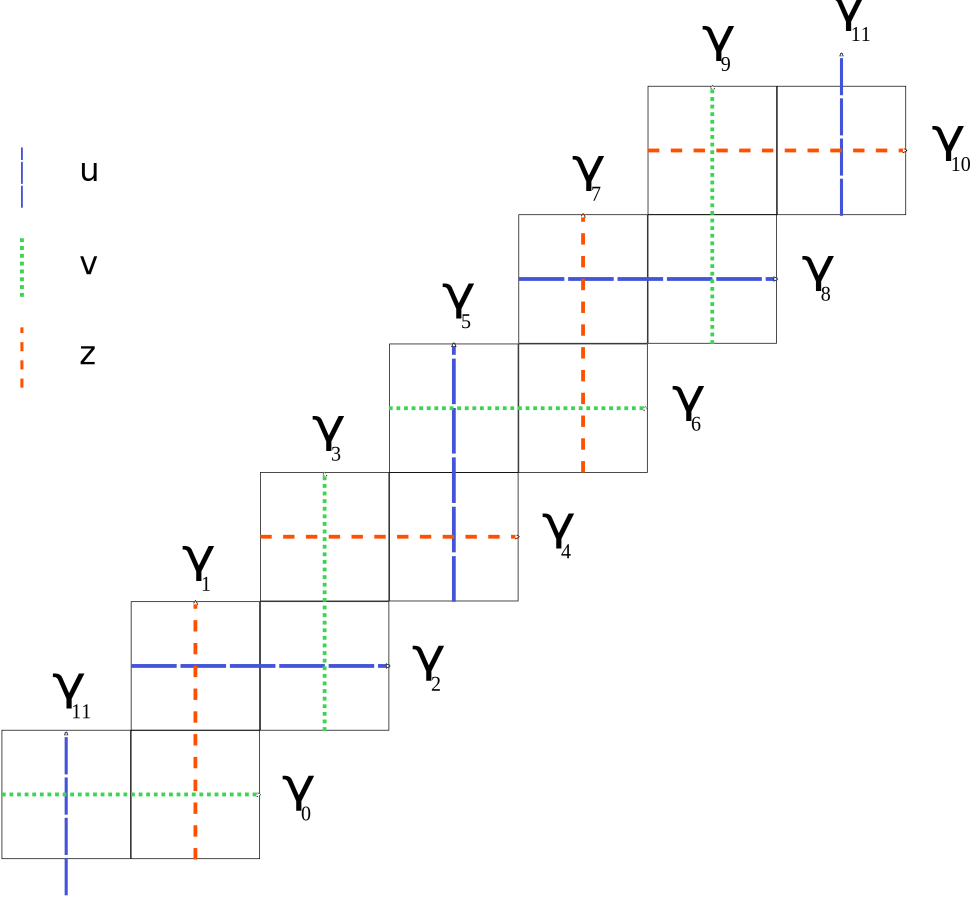
\includegraphics[width=3in]{homologyclass.png}
\centering
\caption{Cylinder core curves with u,v, and z homology classes that determines the $\mathbf{Z}^{2}$-cover.}
\label{fig:homology}
\end{figure}

\begin{Def}
The set of abelianized cylinder core curves is denoted as $\Gamma=\{\gamma_i: i = 0,\dots,11\}\subset H_1(\mathbf{M},\mathbb{Q})$.
\end{Def}

\begin{rem}
We use 12 elements to span homology, although a basis requires only 10. It's not impossible to determine the relations between these core curve classes, but it is not necessary. A $12\times12$ matrix of these core curve cylinder decompositions to their intersection numbers with adjacent curves is rank 10, as to be expected.
\end{rem}

The induced homomorphisms of $H_1(\mathbf{M}, \mathbb Q)$ have come from affine maps that have various effects on these core-curves. We use a 12-gon to represent the set of curves, and show how these elements act on them. The multi-twists add curves to adjacent curves, and the translation maps permute them. The reader is encouraged to check these for themselves.

e.g. for $\mathbf{H,V}\in$Aff$^+(\mathbf{M})$,

\begin{minipage}{0.5\textwidth}
\vspace{0.3in}
\begin{itemize}
\item[\textbf{\emph{$\mathbf{H}$ \& $\mathbf{V}$}}] The effect that these two translations have on the 12-gon is a reflection about these lines. Observed by keeping track of the squares and core curves after $\mathbf{H}$ and $\mathbf{V}$ have acted on $\mathbf{X}$.
\end{itemize}
\end{minipage}
\begin{minipage}{0.7\textwidth}
\begin{figure}[H]
\hspace{0.2in}\includegraphics[width=1.7in]{12gonHV.pdf}
\end{figure}
\end{minipage}

\begin{Def}
The induced homomorphisms of $H_1(\mathbf{M},\mathbb{Q})$ are obtained from the affine subgroup $\mathbb{X}$ and denoted $\mathbb{X}_*$. The associated homomorphisms on the spanning set $\Gamma$ are given as:
\begin{align*}
\mathbf{A}^k_*\circ[\gamma_i]=&[\gamma_i] + \frac{k}{2}(1-(-1)^i)([\gamma_{i-1}]+[\gamma_{i+1}])\\
\mathbf{B}^k_*\circ[\gamma_i]=&[\gamma_i] + \frac{k}{2}(1+(-1)^i)([\gamma_{i-1}]+[\gamma_{i+1}])\\
\mathbf{R}_*\circ[\gamma_i]=&(-1)^i[\gamma_{1-i\text{ mod }12}]\\
\mathbf{H}_*\circ[\gamma_i]=&[\gamma_{12-i\text{ mod }12}]\\
\mathbf{V}_*\circ[\gamma_i]=&[\gamma_{10-i\text{ mod }12}]
\end{align*}
\end{Def}

\begin{Def}
The homology classes $u,v,z$ are given as the following sums of core curves:
\begin{align*}
[u] &= -[\gamma_2] +[\gamma_5] + [\gamma_8] - [\gamma_{11}],\\
[v] &= +[\gamma_0] -[\gamma_3] -[\gamma_6] +[\gamma_9],\\
[z] &= +[\gamma_1] +[\gamma_4]-[\gamma_7]-[\gamma_{10}].
\end{align*}
\end{Def}

\begin{thm}
The fundamental group of the $\mathbb{Z}^2$-cover is obtained by lifting the kernel of the closed paths of $\mathbf{M}$ of the homomorphism:

\begin{align*}
\Omega_{u,v}:\pi_1(\mathbf{M},x_0)\rightarrow \mathbb{Z}^2 \text{; } \beta\mapsto(i(u,[\beta]),i(v,[\beta])),\text{ where}
\end{align*}

\begin{align*}
i:H_1(\mathbf{M},\mathbb Q)\times H_1(\mathbf{M},\mathbb Q)\rightarrow \mathbb Z.
\end{align*}is the intersection number of two homology classes.
\begin{proof}
We know from Theorem $\ref{thm:z2}$ that the translational symmetries of $\tilde{\mathbf{U}}$ induced by $T^{m,n}$ is isometric to $\mathbb{Z}^2$. Since $\mathbf{M}$ is a genus 5 base surface, we know that $\pi_1(\mathbf{M},x_0)\simeq \mathbb{Z}^{10}$, and the associated cover satisfies $\mathbf{M}=\tilde{\mathbf{U}}/(\pi_1(\mathbf{M},x_0)/N)$, such that $N$ is a normal subgroup of $\pi_1(\mathbf{M},x_0)$. This means that $N\simeq \mathbb{Z}^8$. The eight core curve classes are the abelianized forms of  $\gamma_0,\gamma_2,\gamma_3,\gamma_5,\gamma_6,\gamma_8,\gamma_9,$ and $\gamma_{11}$ that span N. The classes and their signs are obtained from Figure $\ref{fig:mtilda}$ as the outer regions identified by the translations of $T^{m,n}$. Thus any closed path on $\mathbf{M}$ is lifted to a closed path on the cover under the quotient map only when a path has a trivial intersection number with the classes.
\end{proof}

\end{thm}
Two paths are homologous if they return the same intersection number with the classes of closed core cylinder curves of $\mathbf{U}$ that span its homology. The classes u and v are obtained from the group group action of $T^{m,n}$ on the cover.

\begin{Def}
$\mathbf{hol}:\mathbf{M}\backslash\text{Sing}(\mathbf{M})\rightarrow\mathbb{C}$ is the holonomy vector pulled back from a non-singular path $\gamma$ in $\mathbf{M}$ onto the complex plane given by $\mathbf{hol}(\gamma)=\int_{\gamma}dz$.
\end{Def}

We denote the \textbf{closed path} $\alpha$, such that $\mathbf{hol}(\alpha)=6+6i$, and show it is homologous to the closed geodesic with the same holonomy vector. The slope one direction also decomposes $\mathbf{M}$ into two cylinders by a series of saddle connections of length $\sqrt{2}$ between singularities:

\begin{figure}[H]
\centering
\includesvg[width=4.4in.]{slopeonecylinder}
\caption{The two right-most cylinders $C_1$ (labeled) and $C_2$(unlabeled).}
\end{figure}

The circumferences of these two cylinders are $6\sqrt{2}$. Geodesic flows on this surface are well defined, and rational directions 

\begin{Def}
Let $\omega^{\theta}_t:[0,1]\times\mathbb{R}/2\pi\mathbb{Z}\rightarrow\mathbf{M}$ be the \textbf{maximal geodesic flow} on the surface in direction $\theta$ such that $\omega^{\theta}_0=\omega^{\theta}_1=x_0\in\mathbf{M}\backslash\text{Sing}(\mathbf{M})$.\\
$\omega^{\frac{\pi}{4}}_t$ is the geodesic flow in the \textbf{slope one direction}, and $\chi$ is its image in $\mathbf{M}$ and element of $\pi_1(\mathbf{M},x_0)$.
\end{Def}

\begin{lem}
$\alpha$ is homologous to $\chi$ in  $\mathbf{M}\backslash\text{Sing}(\mathbf{M})$.
\begin{proof}
Let $\chi$ be a geodesic contained in either $C_1$ or $C_2$. Since a geodesic does not admit singularities, it is the image of a closed path on $X\backslash\text{Sing}(X)$ with initial point $x_0$ on the strips of $C_1$ and $C_2$ with boundaries removed, denoted $C_1',$ $C_2'$. Express $[\alpha]$ as $\Sigma^{11}_{j=0}$ $\frac{1}{2}\gamma_j$ (a closed path climbing up the staircase). We show that the intersection numbers of $[\alpha]$ and $[\chi]$ are the same for every core cylinder curve $\gamma$, i.e. $i([\gamma_k], \Sigma^{11}_{j=0} \text{ } \frac{1}{2}[\gamma_j])=i([\gamma_k],[\chi])\text{ } \forall k=0,\dots,11$.\\
\textbf{Case one:} k is even. If k is even, then every curve $\gamma_k$ is oriented to the right. Since $\chi$ intersects every curve once, $i([\gamma_k],[\chi])=1$. No even indexed curves intersect eachother, so we need only consider when $j$ is odd. Now if $j$ is odd, it is incident (positively crossing) with only two horizontal curves, namely $\gamma_{j+1},\gamma_{j-1}$. Therefore $i([\gamma_k],[\alpha])=i([\gamma_{j-1}],\frac{1}{2}[\gamma_{j}])+i([\gamma_{j+1}],\frac{1}{2}[\gamma_{j}])=\frac{1}{2}(i([\gamma_{j-1}],[\gamma_{j}])+i([\gamma_{j+1}],[\gamma_{j}]))=\frac{1}{2}(1+1)=1.$\\
\textbf{Case two:} k is odd. If k is odd, then $[\chi]$ will have an intersection number of $-1$ with $[\gamma_k]$ since odd-indexed core curves are oriented upwards. Now since k is odd, we only consider when $j$ is even. Similarly, this means that $\gamma_j$ negatively intersects the two vertical core curves with adjacent indices. Hence, $i([\gamma_k],[\alpha])=i([\gamma_{j-1}],\frac{1}{2}[\gamma_{j}])+i([\gamma_{j+1}],\frac{1}{2}[\gamma_{j}])=\frac{1}{2}(i([\gamma_{j-1}],[\gamma_{j}])+i([\gamma_{j+1}],[\gamma_{j}]))=\frac{1}{2}(-1-1)=-1.$\\
We know intersection number to be bilinear and non-degenerate on homology. So if $\alpha$ and $\chi$'s abelianizations admit the same intersection numbers for every curve in the spanning set of $H_1(\mathbf{M}, \mathbb{Q})$, then $[\alpha]=[\chi]$.
\end{proof}
\end{lem}

\begin{thm}
$\chi\in\pi_1(\mathbf{M},x_0)$ lifts to $\tilde{\chi}\in\pi_1(\tilde{\mathbf{U}},\tilde{x}_0)$
\begin{proof}
From Lemma 2, $[\chi]=[\alpha]$, so $\Omega_{u,v}(\chi)=\Omega_{u,v}(\alpha)$. Since
$i([u],[\alpha])=-i([\gamma_2],[\alpha] +i([\gamma_5],[\alpha]) + i([\gamma_8],[\alpha]) - i([\gamma_{11}],[\alpha])=-1+(-1)+1-(-1)=0$ and $i([v],[\alpha])=1-(-1)-1+(-1)=0$, it follows that $\alpha,\chi\in\text{Ker }\Omega_{u,v}$, and $\chi$ lifts to a closed geodesic on $\tilde{\mathbf{U}}$.
\end{proof}
\end{thm}

\begin{cor}
content...
\end{cor}

From here, we use $\alpha$ to show that the \emph{only} trajectories that close on the Necker cube surface are those that are in vector direction $(a,b)$ such that $\gcd(a,b)=1$ and $a,b$ are both odd. We call these \textbf{odd-odd} directions. We can make this claim because the group generated by the matrices 

\begin{equation*}
\left[ \hspace{1mm} \begin{matrix}
				1 &  \pm 2\\
				0 & 1
			\end{matrix}\hspace{1mm}\right] \text{ and }
			\left[ \hspace{1mm} \begin{matrix}
							1 & 0\\
							 \pm 2 & 1
						\end{matrix}\hspace{1mm}\right]
\end{equation*}
is the \emph{Sanov subgroup} of $SL(2,\mathbb{Z})$ and only sends elements in the odd-odd set to itself. There are dualizations made between how these matrices skew a geodesic direction,  and how their original affine transformations induce an effect homology. In a sense the kernel is obtained by the orbit of $\chi$ under $\mathbb{X}$ and its holonomy vector under $\mathbb{X}'$.

\begin{lem}
The actions of $\mathbb{X}'$ on $\mathcal{O}$ and $\mathcal{E}$ are closed in their respective sets.
\begin{proof}
Since $\mathbb{X}'$ is generated by the elements $\mathbf{A}'$, $\mathbf{B}'$, and $\mathbf{R}'$, any matrix $G'\in\mathbb{X}'$ is of the form $G' = (\mathbf{A}')^{1_1}\circ(\mathbf{B}')^{1_2}\circ(\mathbf{R}')^{1_3}\circ(\mathbf{A}')^{2_1}\circ\dots(\mathbf{A}')^{n_1}\circ(\mathbf{B}')^{n_2}\circ(\mathbf{R}')^{n_3}$, where $i_k\in\mathbb{Z}$ for $i=1,\dots,n$ and $k=1,2,3.$ Let $x=\left(\begin{matrix}p \\ q  \end{matrix}\right),y\in\mathcal{O}$, and consider the equation $G'x=y$. Observe that $\left(\begin{matrix}1 && 2 \\ 0 && 1\end{matrix}\right)^l x=\left(\begin{matrix}p+2jq \\ q  \end{matrix}\right),$ and $ \left(\begin{matrix}1 && 0 \\ 2 && 1\end{matrix}\right)^m x=\left(\begin{matrix}p \\ q+2mp  \end{matrix}\right)$ for any $l,m\in\mathbb{Z}$. Also note that for any $j\in\mathbb{Z}$, $(\mathbf{R}')^{m}x=\left(\begin{matrix}p \\ q  \end{matrix}\right),\left(\begin{matrix}-q\\ p  \end{matrix}\right),\left(\begin{matrix}-p \\ -q  \end{matrix}\right),\left(\begin{matrix}q \\ -p  \end{matrix}\right)$ when $j \mod{4}\equiv0,1,2,3$, respectively. In any case, the product of any power of a generator of $\mathbb{X}'$ and any $x\in\mathcal{O}$ is an element of $\mathcal{O}$ . By letting $l=i_1,m=i_2,$ and $j=i_3$, we first consider the base case when $i=n$. Let $G'=G'_1\circ\dots\circ G'_n$, such that $G'_i=(\mathbf{A}')^{i_1}\circ(\mathbf{B}')^{i_2}\circ(\mathbf{R}')^{i_3}$. Since $n_1,n_2,n_3$ are arbitrary integers, $G'_n x \in\mathcal{O}$. Suppose for some $b< n-1$, $G'_{n-b}\circ\dots\circ G'_n x =y'\in\mathcal{O}$. Therefore $y'=(G'_1\circ\dots\circ G'_{b})^{-1}y$, which implies that $(G'_1\circ\dots\circ G'_{b})^{-1}$ preserves the set $\mathcal{O}$. Otherwise, if $y\in\mathcal{E}$, there exists at least one $G'_i$ for $1< i< b$ and $\tau\in\mathcal{E}$ such that $G'^{-1}_i \tau = (\mathbf{R}')^{-i_3}\circ(\mathbf{B}')^{-i_2}\circ(\mathbf{A}')^{-i_1} \tau \in \mathcal{O}$, a contradiction. Since elements in $\mathbb{X}'$ are invertible, $G'_1\circ\dots\circ G'_{b}$ must also map $\mathcal{O}$ to itself. Left multiply both sides of the equation to show that $G'_1\circ\dots\circ G'_n x = G' x = y$. By the principle of strong induction, this holds for all $0<b\leq n$. Since $G'$ is invertible and an arbitrarily chosen element of $\mathbb{X}'$, it follows that $x\in\mathcal{O}$ if and only if $y\in\mathcal{O}$ and $\mathcal{O}$ is closed under $\mathbb{X}'$.\\
The proof for when $x\in\mathcal{E}$ is made in the same way.
\end{proof}
\end{lem}


Now a trajectory in the horizontal direction has a directional vector of (1,0). The orbit of this vector by the Veech group is the set of all \textbf{even-odd} vectors. We also know that in this direction a geodesic is drift-periodic (See figure 1). The Veech group of $\mathbf{M}$ preserves these properties. Suppose you had some closed geodesic on $\mathbf{M}\backslash Sing(\mathbf{M})$ called $\beta$ such that $\beta=h(\alpha)$, where $h\in$  Aff$^+(\mathbf{M})$, and $h_*$ is its induced homomorphism. Then we want to show that

\begin{align*}
(i([\beta],[u]), i([\beta],[v]))=(i([\alpha],h^{-1}_*[u]), i([\alpha],h^{-1}_*[v])) = (0,0).
\end{align*}

But first, we look at some of the properties of the group $\mathbb{X}_*$.

\begin{thm}
Let $\mathbb{X}_*$ be the group generated by $\mathbf{A}_*, \mathbf{B}_*, \mathbf{R}_*, \mathbf{H}_*,$ and $\mathbf{V}_*$. Let $G=\left< \mathbf{A}_*, \mathbf{B}_* \right>$, $T=\left< \mathbf{H}_*, \mathbf{V}_* \right>$, and $R=\left< \mathbf{R}_*\right>$. Then the following is true:
\begin{enumerate}[label=(\roman*)]
\item $G$ is a free subgroup of $\mathbb{X}_*$ of rank two.
\item $T$ is a finite cyclic subgroup of $\mathbb{X}_*$ and a centralizer of G.
\item $R$ is a finite cyclic subgroup of $\mathbb{X}_*$, and a normalizer of $G$.
\end{enumerate}
\begin{proof} Let $h_*^{j}=\mathbf{A}_*^{k_j}\circ \mathbf{B}_*^{g_j}\in G$ for $k_j, g_j \in\mathbb{Z}$, $j=1,\dots,n$.\\ \emph{(i)}. When $\mathbf{A}_*$ and $\mathbf{B}_*$ act on $\gamma_i$, it is only ever trivial if i is even for $\mathbf{A}_*$ or i is odd on $\mathbf{B}_*$. Since i cannot be both odd and even at the same time, there is no relation between the two generators and therefore $G$ is free.\\
\emph{(ii)} It is up to the reader to show that $T$ has the relations $\mathbf{H}_*^2=\mathbf{V}_*^2=(\mathbf{H}_*\mathbf{V}_*)^3=id_*$, and is isomorphic to the rotational group of the hexagon generated by reflections about adjacent vertices of a 12-gon. Observe that $\mathbf{H}_*\circ \mathbf{A}_*^{k_j}\circ[\gamma_i]=\mathbf{H}_*\circ[\gamma_i] + \frac{k_j}{2}(1-(-1)^i)(\mathbf{H}_*\circ[\gamma_{i-1}]+\mathbf{H}_*\circ[\gamma_{i+1}])=[\gamma_{-i}] + \frac{k_j}{2}(1-(-1)^i)([\gamma_{1-i}]+[\gamma_{-i-1}])=\mathbf{A}^{k_j}\circ[\gamma_-i]=\mathbf{A}^{k_j}\circ\mathbf{H}_*\circ[\gamma_i],$ and $\mathbf{V}_*\circ \mathbf{A}_*^{k_j}\circ[\gamma_i]=\mathbf{V}_*\circ[\gamma_i] + \frac{k_j}{2}(1-(-1)^i)(\mathbf{V}_*\circ[\gamma_{i-1}]+\mathbf{V}_*\circ[\gamma_{i+1}])=[\gamma_{10-i}] + \frac{k_j}{2}(1-(-1)^i)([\gamma_{11-i}]+[\gamma_{9-i}])=\mathbf{A}^{k_j}\circ[\gamma_10-i]=\mathbf{A}^{k_j}\circ\mathbf{V}_*\circ[\gamma_i].$ In the same way one can show this to be true for $\mathbf{B}_*^{g_j}$, and we can see that $T$ is a centralizer of $G$. \\
\emph{(iii)} $R$ is obviously cyclic and finite since an isomorphism is obtained as $\mathbf{R}_*\mapsto\mathbf{R}'\in SO(2,\mathbb{Z})$. \\Note that $\mathbf{R}_*\circ\mathbf{A}_*^{k_j}\circ[\gamma_i]=\mathbf{R}_*\circ[\gamma_i] + \frac{k_j}{2}(1-(-1)^i)(\mathbf{R}_*\circ[\gamma_{i-1}]+\mathbf{R}_*\circ[\gamma_{i+1}])\\
=(-1)^i[\gamma_{1-i}] + \frac{k_j}{2}(1-(-1)^i)((-1)^{i-1}[\gamma_{2-i}]+(-1)^{i+1}[\gamma_{-i}])\\
=(-1)^{1-i}([\gamma_{1-i}] - \frac{k_j}{2}(1+(-1)^{1-i})([\gamma_{2-i}]+[\gamma_{-i}]))\\
=(-1)^{1-i}\mathbf{B}_*^{-k_j}\circ[\gamma_{1-i}]=\mathbf{B}_*^{-k_j}\circ(-1)^{1-i}[\gamma_{1-i}]=\mathbf{B}_*^{-k_j}\circ\mathbf{R}_*\circ[\gamma_{i}].$\\
Likewise, $\mathbf{R}_*\circ\mathbf{B}_*^{g_j}\circ[\gamma_{i}]=\mathbf{A}_*^{-g_j}\circ\mathbf{R}_*\circ[\gamma_{i}]$.
\end{proof}
\end{thm}

\begin{rem}
It can be easily shown that $\mathbb{X}'$ has similar properties.
\end{rem}


\begin{lem}
$Let$ $h_*\in \left<\mathbf{A}_*,\mathbf{B}_*\right>. $ Then $h_*\circ[\alpha]\in H_1(\mathbf{M},\mathbb{Q})$ can be expressed as $h_*\circ[\alpha]=\frac{1}{2}(c_1\Sigma^{5}_{j=0}[\gamma_{2j}]+c_2\Sigma^{5}_{j=0}[\gamma_{2j+1}])$ for $c_1,c_2\in\mathbb{Z}$.
\begin{proof}
Let $\Sigma^{5}_{j=0}[\gamma_{2j}]=\Sigma\Gamma_{even}$, $\Sigma^{5}_{j=0}[\gamma_{2j+1}]= \Sigma\Gamma_{odd}$, and  $\Sigma^{11}_{j=0}[\gamma_{j}]= \Sigma\Gamma$. Let $h_*=h_*^n\circ\dots\circ h_ *^1$, and $h_*^{i}=\mathbf{A}_*^{k_i}\circ \mathbf{B}_*^{g_i}$ for $k_i, g_i \in\mathbb{Z}$, $i=1,\dots,n$. Compose these two homomorphisms and obtain $\mathbf{A}_*^{k_i}\circ \mathbf{B}_*^{g_i}(\Sigma\Gamma)=(4g_ik_i+2k_i)\Sigma\Gamma_{even}+2g_i\Sigma\Gamma_{odd}+\Sigma\Gamma$. Let $c_i^1=(4g_ik_i+2k_i), c_i^2=2g_i$, and solve for $h_*^{i+1}\circ h_*^i\circ\Sigma\Gamma$:
\begin{align*}
h_*^{i+1}\circ h_*^{i}\circ(\Sigma\Gamma)=h_*^{i+1}\circ(c_i^1\Sigma\Gamma_{even}+c_i^2\Sigma\Gamma_{odd}+\Sigma\Gamma)\\ =c_i^{1}h_*^{i+1}\circ(\Sigma\Gamma_{even})+c_i^2h_*^{i+1}\circ(\Sigma\Gamma_{odd})+h_*^{i+1}\circ(\Sigma\Gamma)\\ =2g_{i+1}\Sigma\Gamma_{odd}+(4g_{i+1}k_{i+1}+2k_{i+1})\Sigma\Gamma_{even}+\Sigma\Gamma\\+c_i^{1}(4g_{i+1}k_{i+1}\Sigma\Gamma_{even}+2g_{i+1}\Sigma\Gamma_{odd}+\Sigma\Gamma_{even})\\+c_{i}^2(2k_{i+1}\Sigma\Gamma_{even}+\Sigma\Gamma_{odd})\\
=\Sigma\Gamma+(c_i^1+(c_{i}^1+1)(4g_{i+1}k_{i+1})+(c_i^2+1)2k_{i+1})\Sigma\Gamma_{even}\\+(c_i^2+(c_i^1+1)2g_{i+1})\Sigma\Gamma_{odd}\\
\text{Let }c_{i+1}^1:=(c_i^1+(c_{i}^1+1)(4g_{i+1}k_{i+1})+(c_i^2+1)2k_{i+1}),\\
c_{i+1}^2:=(c_i^2+(c_i^1+1)2g_{i+1}).
\end{align*}
From these recursive definitions and a finite sequence of integers, $\{k\}_i,\{g\}_i$, observe then that\\ $h_*\circ[\alpha]=h_*\circ[\frac{1}{2}\Sigma\Gamma]=\frac{1}{2}h_*\circ[\Sigma\Gamma]=\frac{1}{2}[c_n^1\Sigma\Gamma_{even}+c_n^2\Sigma\Gamma_{odd}+\Sigma\Gamma]\\
=\frac{1}{2}[(c_n^1+1)\Sigma\Gamma_{even}+(c_n^2+1)\Sigma\Gamma_{odd}]$. Further simplify by letting $c_1=c_n^1+1,c_2=c_n^2+1$.
\end{proof}
\end{lem}

\begin{lem}
Let $h_*\circ[\alpha]\in H_1(\mathbf{M},\mathbb{Q})$. Then for $a\in\left<\mathbf{H}_*, \mathbf{V}_*\right>$ and $b\in\left<\mathbf{R}_*\right>$, the following is true:
\begin{align*}
& a\circ h_*\circ[\alpha]=h_*\circ[\alpha]\\
& b\circ h_*\circ[\alpha]=\frac{1}{2}[c'_1\Sigma\Gamma_{even}+c'_2\Sigma\Gamma_{odd}]\\
& h_*\circ b\circ[\alpha]=\frac{1}{2}[c''_1\Sigma\Gamma_{even}+c''_2\Sigma\Gamma_{odd}]
\end{align*}
\begin{proof}
By Theorem 4, a is a centralizer of the group so $a\circ h_*\circ[\alpha]=h_*\circ a \circ[\alpha]=h_*\circ \frac{1}{2}a \circ[\Sigma\Gamma].$ Since a is a cyclic permutation of the set $\Gamma$, it acts trivially on $\Sigma\Gamma$. Therefore, $a\circ h_*\circ[\alpha]=h_*\circ \frac{1}{2}[\Sigma\Gamma]=h_* \circ[\alpha]$.\\
By theorem 4, $a\circ\mathbf{A}_*^{k_i}\circ\mathbf{B}_*^{g_i}=\mathbf{B}_*^{-k_i}\circ\mathbf{A}_*^{-g_i}\circ a$. Extend this property to $h_*$, and denote the normalized element as $h_{**}$, such that $b\circ h_{*}=h_{**}\circ b$.  Note that $b(\Sigma\Gamma)=b(\Sigma\Gamma_{even}+\Sigma\Gamma_{odd})=\Sigma\Gamma_{odd}-\Sigma\Gamma_{even}$. $b\circ h_*\circ[\Sigma\Gamma]=c_1b\circ\Sigma\Gamma_{even}+c_2b\circ\Sigma\Gamma_{odd}=c_1\Sigma\Gamma_{odd}-c_2\Sigma\Gamma_{even}.$ So, $c_1'=-c_2$ and $c_2'=c_1$.\\
Since $h_*$ is arbitrary, let $h_{**}=g_{*}$ be generated by an integer sequence that defines the word and consider $h_*\circ b\circ[\Sigma\Gamma]=b\circ g_{*}\circ[\Sigma\Gamma]=c^*_1b\circ\Sigma\Gamma_{even}+c^*_2b\circ\Sigma\Gamma_{odd}=c^*_1\Sigma\Gamma_{odd}-c_2^*\Sigma\Gamma_{even}.$ So, $c_1''=-c_2^*$ and $c_2''=c_1^*$.
\end{proof}
\end{lem}

\noindent Now that every element in the orbit of $[\alpha]$ can be expressed as a linear combination of integers, it is simple to show they lift to a closed trajectory in the cover.

\begin{Def}
Let $\mathbf{dir}:UT(\mathbf{M}\backslash\text{Sing}(\mathbf{M}))\rightarrow\mathcal{O}\cup\mathcal{E}$ be the injective map from $\mathbb{R}/2\pi\mathbb{Z}$ to $\mathbb{Z}^2$ given as $\mathbf{dir}(\theta)=(k_1\cos(\theta),k_2\sin(\theta)), k_1,k_2\in\mathbb{R}$ such that $\gcd(k_1\cos(\theta),k_2\sin(\theta))=1$.
\end{Def}

\begin{thm}(Sketch)\\
Any geodesic, $\beta$, in $\mathbf{M}$ lifts to a closed geodesic $\tilde{\beta}$ on $\tilde{\mathbf{U}}$ if and only if $\mathbf{dir}(Arg(\mathbf{hol}(\beta)))\in\mathcal{O}$.
\begin{proof}
Call the quotient cover $p:\tilde{\mathbf{U}}\rightarrow\mathbf{M}$, and fix a point $\tilde{x_0}\in p^{-1}(x_0)$. Let $\beta=h(\chi)$, where $h\in\mathbb{X}$. We also obtain $[\beta]=h_*\circ[\alpha]$ from Lemma 2. Since $h$ sends geodesics to geodesics, h induces the following: $\mathbf{hol}(h(\chi))=h'(\mathbf{hol}(\chi))=h'(6+6i)$ for $h'=\left[\begin{matrix} a & b \\ c & d\end{matrix}\right]\in\mathbb{X}'$. So, Arg$(h'(\mathbf{hol}(\chi)))=$Arg$(6[(a+b)+i(c+d)])=$Arg$(6h'(1+i))$. Lemma 3 states that for any $h'\in\mathbb{X}'$, $h'(\mathcal{O})=\mathcal{O}$. Therefore there is no such geodesic of \textbf{even-odd} slope in the orbit of $\chi$. Otherwise $h',h\notin\mathbb{X}',\mathbb{X}$. Consequently, $\mathbf{dir}(Arg(\mathbf{hol}(\beta)))\in\mathcal{O}$.\\
From Lemma 5 we see that $[h(\chi)]=h_*\circ[\chi]=h_*\circ[\alpha]=\frac{1}{2}(c_1\Sigma^{5}_{j=0}[\gamma_{2j}]+c_2\Sigma^{5}_{j=0}[\gamma_{2j+1}])$ for $c_1,c_2\in\mathbb{Z}$. Denote the sums as $\Sigma\Gamma_{even}$ and $\Sigma\Gamma_{odd}.$\\
Therefore, $2i([u],h_*\circ[\alpha])=c_1i([u],\Sigma\Gamma_{even})+c_2i([u],\Sigma\Gamma_{odd})\\
=c_1(-i([\gamma_2],0) +i([\gamma_5],[\gamma_6]+[\gamma_4]) + i([\gamma_8],0) - i([\gamma_{11}],[\gamma_{10}]+[\gamma_{0}]))\\
+c_2(-i([\gamma_2],[\gamma_1]+[\gamma_3]) +i([\gamma_5],0) + i([\gamma_8],[\gamma_7]+[\gamma_9]) - i([\gamma_{11}],0))\\
=c_1(-(0)+(-1-1)+(0)-(-1-1))+c_2(-(1+1)+(0)+(1+1)-(0))=0.$\\\vspace{0.1in}\\
Similarly, $2i([v],h_*\circ[\alpha])=c_1i([v],\Sigma\Gamma_{even})+c_2i([v],\Sigma\Gamma_{odd})\\
=c_1(i([\gamma_0],0)-i([\gamma_3],[\gamma_2]+[\gamma_4])-i([\gamma_6],0)+i([\gamma_9],[\gamma_8]+[\gamma_{10}])\\
+c_2(i([\gamma_0],[\gamma_{11}]+[\gamma_1])-i([\gamma_3],0)-i([\gamma_6],[\gamma_5]+[\gamma_7])+i([\gamma_9],0)\\
=c_1((0)-(-2)-(0)+(-2))+c_2((2)-(0)-(2)+(0))=0.$\\
Therefore, $\Omega_{u,v}(h(\chi))=(0,0)$, and $h(\chi)=\beta\in\text{Ker }\Omega_{u,v}$ for all $h\in\mathbb{X}$. By Theorem 2, $\beta$ lifts to $\tilde{\beta}\in\pi_1(\tilde{\mathbf{U}},\tilde{x}_0)$. Let $\theta=$Arg$(\mathbf{hol}(\beta))$. Then $\omega_t^{\theta}$ at $x_0$ lifts to $\tilde{\omega}_t^{p^{-1}(\theta)}\in\tilde{\mathbf{U}}\backslash\text{Sing}(\tilde{\mathbf{U}})$.\\
Now suppose instead that $\beta=h(\gamma_{i})$. Then $\mathbf{dir}(\beta)=\frac{1}{2}(1+(-1)^i,1-(-1)^i)$. According to Lemma 3, $h'(\mathcal{E})=\mathcal{E}$. Thus we have no geodesic in the \textbf{odd-odd} directions obtained from the orbits of $(1,0)$ and $(0,1)$. For contradiction, suppose that $h(\gamma_{i})\in\textbf{Ker }\Omega{u,v}$. Then $(i(h_*\circ[\gamma_i], [u]),i(h_*\circ[\gamma_i], [v]))=(i([\gamma_i], h^{-1}_*\circ[u]),i([\gamma_i], h^{-1}_*\circ[v]))=(0,0).$ Let $h^{-1}_*\circ[u]=\Sigma^{11}_{j=0}x_j[\gamma_j]$, and $h^{-1}_*\circ[v]=\Sigma^{11}_{j=0}y_j[\gamma_j]$. Note that since $\gamma_i$ intersects $\gamma_{i\pm1}$, $i([\gamma_i], h^{-1}_*\circ[u])=(-1)^{i+1}(x_{i-1}+x_{i+1})$ and $i([\gamma_i], h^{-1}_*\circ[v])=(-1)^{i+1}(y_{i-1}+y_{i+1}).$
\\
$\mathbf{Unfinished.}.$
\end{proof}
\end{thm}

\begin{conj}{\textbf{Dynamics of Geodesic Flow on the Necker cube surface.}}\\ Obtain $\theta$ and $\vec{\theta}$ as described in Definition 3. Denote the non-singular unit-speed geodesic flow with initial point $s\in(\mathbf{U}\backslash Sing(U))$ in direction $[\theta]\sim\phi\in UT(\mathbf{U}\backslash Sing(\mathbf U))$ by $F_t^{\phi}:\mathbf{U}\times\mathbb{R}_0^+\rightarrow\mathbf{U}$ on $(\mathbf{U},\mu)$, where $\mu$ is a flow-invariant measure.  Then the following is true:
\begin{enumerate}[label=(\roman*)]
\item (Periodic) There exists a $t_0 > 0$ such that $F^{\phi}_{t+t_{0}}(s)=F^{\phi}_{t}(s)$ if and only if $\vec{\theta}\in\mathcal{O}$.
\item (Drift-Periodic) There exists a $t_0 > 0$ such that $F^{\phi}_{t+t_{0}}(s)= F^{\phi}_{t}(s)+c$, where $c\in \mathbf{U}$ is a non-trivial translation of a point in $\mathbf{U}$, if and only if $\vec{\theta}\in\mathcal{E}$.
\end{enumerate}
\begin{proof}(Sketch)\\
Denote the covering maps $f:\tilde{\mathbf{U}}\rightarrow\mathbf{U}$, $p:\tilde{\mathbf{U}}\rightarrow\mathbf{M}$, and fix a point $\tilde{x}_0\in f^{-1}(s),p^{-1}(x_0),$ for $x_0\in\mathbf{M}$. $f^{-1}([\theta])=\{x:x=\theta+n\frac{\pi}{2}, n\in\mathbb{Z}\}=[\theta]\subset UT(\tilde{\mathbf{U}}\backslash\text{Sing}(\tilde{\mathbf{U}}))$ given by the four-fold cover and rotations of each individual plane. This gives us a relation between the two tangent bundles, where the translation four-fold cover has the standard $\mathbb{R}/2\pi\mathbb{Z}$ unit tangent fiber. $\theta'$ is the direction associated to the flow $\omega_t^{\theta'}:[0,1]\rightarrow\mathbf{M}$ on the translation surface. Since the cover is translation, $p^{-1}(\theta')=\theta'=\theta+n\frac{\pi}{2}$.  First suppose that $\vec{\theta}\in\mathcal{O}$. Then $\theta$ is identified with the set of directions that close on $\tilde{\mathbf{U}}$. From Theorem 5, $\omega_t^{\theta'}$ lifts to a closed geodesic $\tilde{\omega}_t^{\theta'}$. Given $\mathbf{hol}(\omega)=\int_{\omega}dz$, we obtain a period for the unit-speed flow, $t_0=|\mathbf{hol}(\omega)|$. That is, $\tilde{F}_t^{\theta'}:\mathbb{R}^+_0\rightarrow\tilde{\mathbf{U}}$ such that  $\frac{d}{dt}\tilde{F}_t=\frac{1}{|\mathbf{hol}(\omega)|}$. Then $F_t^{\phi}=F_t^{[\theta']}=f\circ \tilde{F}^{\theta'}_t$. The period carries over since there is no concern over a trajectory returning to $\tilde{x_0}$ in a different direction. Otherwise, the geodesic $\omega_t^{\theta'}$ on $\mathbf{M}$ would have closed in $0<t<1$. Now suppose that $\vec{\theta}\in\mathcal{E}$. Identifying it with $\theta'$, we see that $\omega$ in direction $\theta'$ is not an element of $\textbf{Ker }\Omega_{u,v}$ from Theorem 5. Therefore, $\Omega_{u,v}(\omega)=(m,n)\simeq T^{m,n}$ and lifting the terminal point $\omega(1)$, $\tilde{\omega}(1)=T^{m,n}(\tilde{\omega}(0))=T^{m,n}(\tilde{x}_0).$ The period remains unchanged, in that $\tilde{F}^{\theta'}_{t+\mathbf{hol}(\omega)}=\tilde{F}^{\theta'}_{t}+T^{m,n}(\tilde{x}_0)$. Therefore, $F^{\phi}_{t+t_{0}}(s)=f\circ\tilde{F}^{\theta'}_{t}(\tilde{x}_0)+f\circ T^{m,n}(\tilde{x}_0).$\\
Conversely, suppose $F_t$ is periodic. Then $[\theta]=\phi=[\theta']$, which defines directional flows $\tilde{F}^{\phi}_t$. According to Theorem 5, $\tilde{F}^{\phi}_t$ will close if and only if $\phi\subset\mathcal{O}$. $\phi$ is the orbit of $\vec{\theta}'$ under the 90 degree rotational matrix. This matrix does not alter the length or period of a geodesic. Thus, $F^{\phi}_t$ is exactly one of the flows $\tilde{F}^{\phi}_t$. Likewise, if $F^\phi_t$ is drift-periodic then $F^\phi_{t+t_0}=f\circ \tilde{F}^\phi_t+f\circ T^{m,n}$. $T^{m,n}$ is trivial if and only if $\theta'\in\mathcal{O}$. Therefore, $\theta'\in\mathcal{E}$, and $[\theta']=\phi$.
\end{proof}
\end{conj}

There is still much work to do in terms of cleaning up the proofs and organizing the final paper.

\newpage
\section*{Conclusion}
What I ultimately aim to do is port these results on X's homology back to the Necker cube surface. I want do it in such a way that the final theorem is bi-conditional. To do so, I imagine I can take a vector image of a small segment of a geodesic in $\mathbb{R}^3$ and project it onto the isometric flattening of the Necker Cube surface to obtain a direction (or classes of equivalent directions), and relate it to the unit tangent bundle of $\mathbf{M}$.

In addition, I would also like to find a formula for the arc-length of a geodesic based on direction alone. Knowing that hol$(\alpha)=6+6i$ means that the induced Euclidean metric on $\mathbf{M}\backslash$Sing($\mathbf{M}$) gives the geodesic an arc-length of $6\sqrt{2}$. I would like to show that:

\begin{align*}
\int_{\beta}|dz|=|hol(h(\alpha))|=|h'(hol(\alpha))|,
\end{align*}
\noindent where $h'\in V(\mathbf{M})$ is the derivative of h, and $\beta=h(\alpha)$. We know that is true on the translation surface, but it's a matter of then showing the translation quotient, branch-cover, and the Necker cube surface have the same induced Euclidean metric of these non-singular geodesics. (It would not be surprising considering that the surface is built out of subsets of planes.) Even more of a problem is finding a way to solve for a matrix in the Sanov subgroup that brings (1,1) to the desired odd-odd slope.



\newpage
\begin{thebibliography}{9}
\bibitem{Necker} 
\bibitem{Albert} Necker, L.A., \emph{Observations on some remarkable optical phaenomena seen in Switzerland; and on an optical phaenomenon which occurs on viewing a figure of a crystal or geometrical solid.} London and Edinburgh Philosophical Magazine and Journal of Science. 1832. doi:10.1080/14786443208647909
\bibitem{Qbert} Gottlieb., \emph{Q*bert} [Arcade], Gottlieb, 1982.
\bibitem{Escher1} Escher, M.C., \emph{Metamorphosis I}, 1937.
\bibitem{Escher2} Escher, M.C., \emph{Convex and Concave}, 1955.
\end{thebibliography}
\end{document}          
